	
\documentclass[journal ]{new-aiaa}
%\documentclass[conf]{new-aiaa} for conference papers
\usepackage[utf8]{inputenc}
\usepackage{textcomp}

\usepackage{graphicx}
\usepackage{amsmath}
\usepackage[version=4]{mhchem}
\usepackage{siunitx}
\usepackage{longtable,tabularx}
\usepackage{algpseudocode,algorithm,algorithmicx}

%\usepackage{longtable}
\usepackage{supertabular}
\setlength\LTleft{0pt} 


\title{Sun-Avoidance Slew Planning with Keep-Out Cone and  Actuator Constraints}

\author{Mohammad A. Ayoubi \footnote{Associate Professor, Department of Mechanical Engineering, Santa Clara University, 500 El Camino Real, Santa Clara, CA 95053, AIAA Senior Member.} }
\affil{Santa Clara University, 500 El Camino Real, Santa Clara, CA 95053 }
\author{Junette Hsin\footnote{Engineer, Dynamics and Control Analysis Group, Maxar Space Infrastructure (formerly Space Systems/Loral), 3825 Fabian Way, Palo Alto, CA 94303.}}
\affil{Maxar Space Infrastructure (formerly Space Systems/Loral), 3825 Fabian Way, Palo Alto, CA 94303}

\begin{document}

\maketitle
				
	\begin{abstract}
This paper presents a geometric approach for a Sun (or any bright object) avoidance slew maneuver with pointing and actuator constraints. We assume that a gyrostat has a single light-sensitive payload with control-torque and reaction wheels' angular momentum constraints. Furthermore, we assume that the initial and final attitudes, an instrument's line-of-sight (LOS) vector, and sun vector are known. Then we use Pontryagin's minimum principle (PMP) and derive the desired or target-frame quaternions, angular velocity and acceleration. In the end, a Monte Carlo simulation is performed to show the viability of the proposed algorithm with control-torque and angular momentum constraints. 
% for two cases: 1) with control-torque and reaction wheels' angular momentum constraints, and 2) with control-torque. constraint.  		
	\end{abstract}
\section*{Nomenclature}

%\noindent(Nomenclature entries should have the units identified)
{\renewcommand\arraystretch{1.0}
\noindent\begin{longtable*}{@{}l @{\quad=\quad} l@{}}
		
		$\hat{e}$ & unit vector along eigenaxis \\ 
		$H$ & the total angular momentum of the gyrostat with respect to its center-of-mass \\ 
		$h$ & the total angular momentum of reaction wheel with respect to its center-of-mass  \\ 
		$I$ &the mass-moment-of-inertia of the gyrostat\\ 
%		$I^{w/w*}$ & the mass-moment-of-inertia of reaction wheels with respect to their center of masses\\ \\
		$\hat{P}$ & unit position vector \\ 
		$q$& quaternion of one frame with respect to the other frame\\ 
		$\hat{S}$ & unit sun vector\\ 
		$\epsilon$ & instrument half-cone angle\\ 	
		$\alpha$& the angle between the sun vector and the slew plane\\ 
		$\omega$& angular velocity of gyrostat\\ 
		\multicolumn{2}{@{}l}{Subscripts or superscripts}\\
		$\mathcal{G}$-frame& gyrostat body-fixed frame \\ 
		$\mathcal{G^*}$& gyrostat center-of-mass \\ 
		$\mathcal{N}$-frame & the Newtonian frame \\ 
		$p$ & Payload \\ 
		$\mathcal{T}$-frame & the target frame \\ 
		$w$ & reaction wheel frame \\ 
		$w*$ & reaction wheel center-of-mass \\ 

\end{longtable*}}
	\section{Introduction}
	\lettrine{L}{arge}-angle slew maneuvers are required during any Earth-pointing or interplanetary missions. In many space missions, and for safety considerations, a sensitive payload such as an imaging camera or telescope needs to be retargeted while avoiding the sun vector or other bright objects in the sky.
	
	The attitude reorientation problem in the presence of attitude constrained zones has been studied in the last three decades. McInnes\cite{McInnes1994} addressed this problem via an artificial potential function. He proposed an entirely analytical guidance law which was suitable for onboard implementation. However, he used Euler angles, which are singular for large slew angles. 
	A geometric approach was proposed by Spindle\cite{Spindler1998}, Hablani\cite{Hablani1998}, and Biggs and Colley\cite{Biggs2016}  where a feasible attitude maneuver, or a guidance law, is precomputed based on the attitude-avoidance-zone constraints.  Another approach for addressing this problem used randomized algorithms\cite{Frazzoli01}. However, depending on the number of constraints and initial and final attitudes, this approach can be computationally expensive and not suitable for onboard implementation. Another approach for solving the time optimal reorientation maneuver subject to boundaries and path constraints was proposed by Spiller et al.\cite{Spiller2016}. They used the particle swarm optimization (PSO) technique to find a sub-optimal solution with keep-out constraints. Another approach casted the problem as a convex optimization problem and used semi-definite programming (SDP) or quadratically constrained quadratic programming (QCQP) in its solution (see for instance Kim and Mesbahi\cite{Kim2004}, Kim et al.\cite{Kim2010}, Sun and Dai\cite{Sun2015}, and Lee and Mesbahi\cite{Lee2014}). Recently, Ramos and Schaub\cite{Ramos2018} proposed a method based on the Lyapunov stability theorem and logarithmic barrier potential function to derive a steering law for attitude control of a gyrostat subject to conically constrained inclusion and exclusion regions. They also considered the control-torque constraint in their algorithm.  
	
In this paper, we present a novel geometric approach for large-angle slew planning with pointing and actuator constraints.  We assume that the gyrostat has a single light-sensitive payload with control-torque and reaction wheels' angular momentum constraints. Furthermore, we assume that the initial and final attitudes, instrument's LOS vector, and sun vector are known. Then, we derive the desired or target-frame quaternions, angular velocities, and angular accelerations based on the Pontryagin's minimum principle (PMP) for the proposed maneuver. The proposed algorithm in this paper is intuitive, deterministic, easy to implement, and includes the control-torque and reaction wheels' angular momentum constraints. The main drawback of the proposed algorithm is its limitation for a single sensitive-payload.  A Monte Carlo simulation is performed to show the viability of the proposed algorithm with control-torque and angular momentum constraints. 
	
%-------------------------------------------------------------------------------------------------------------------------------------------------------------------
\section{Problem Formulation}
Consider a gyrostat, (a rigid body with reaction wheels) and let us define a Newtonian frame, $N$, and a gyrostat-centered unit sphere frame $G$ with a center $G^*$ as shown in Fig. ~1. The sun or bright-object avoidance planning problem can be stated as follows: 

Assume the initial state, $x_i=\big[_\mathcal{N}\hat{P}_i$, $^\mathcal{N}_\mathcal{G}\omega^\mathcal{G}(t_i)$, $^\mathcal{N}q^\mathcal{G}(t_i)\big]\in \mathbb{R}^3\times \mathbb{R}^3\times \mathbb{SO}(3)$, final state, $x_f=$\big[$_\mathcal{N}\hat{P}_f$, $^\mathcal{N}_\mathcal{G}\omega^\mathcal{G}(t_f)$, $^\mathcal{N}q^\mathcal{G}(t_f)\big]\in \mathbb{R}^3\times \mathbb{R}^3\times \mathbb{SO}(3)$, the sun unit vector in the $\mathcal{N}$-frame, $_\mathcal{N}\hat{S}\in \mathbb{R}^3$, the sensitive instrument's LOS unit vector in the $\mathcal{G}$-frame, $_\mathcal{G}\hat{P}\in \mathbb{R}^3$, and the half-cone angle $\epsilon_p\in \mathbb{R}$ are given. Find a sequence of slew maneuvers such that the sun vector does not enter into the on-board sensitive instrument forbidden cone for all times $t\in [t_i, t_f]$ subject to actuator constraints.
		\begin{figure}[htb]
			\begin{center}
				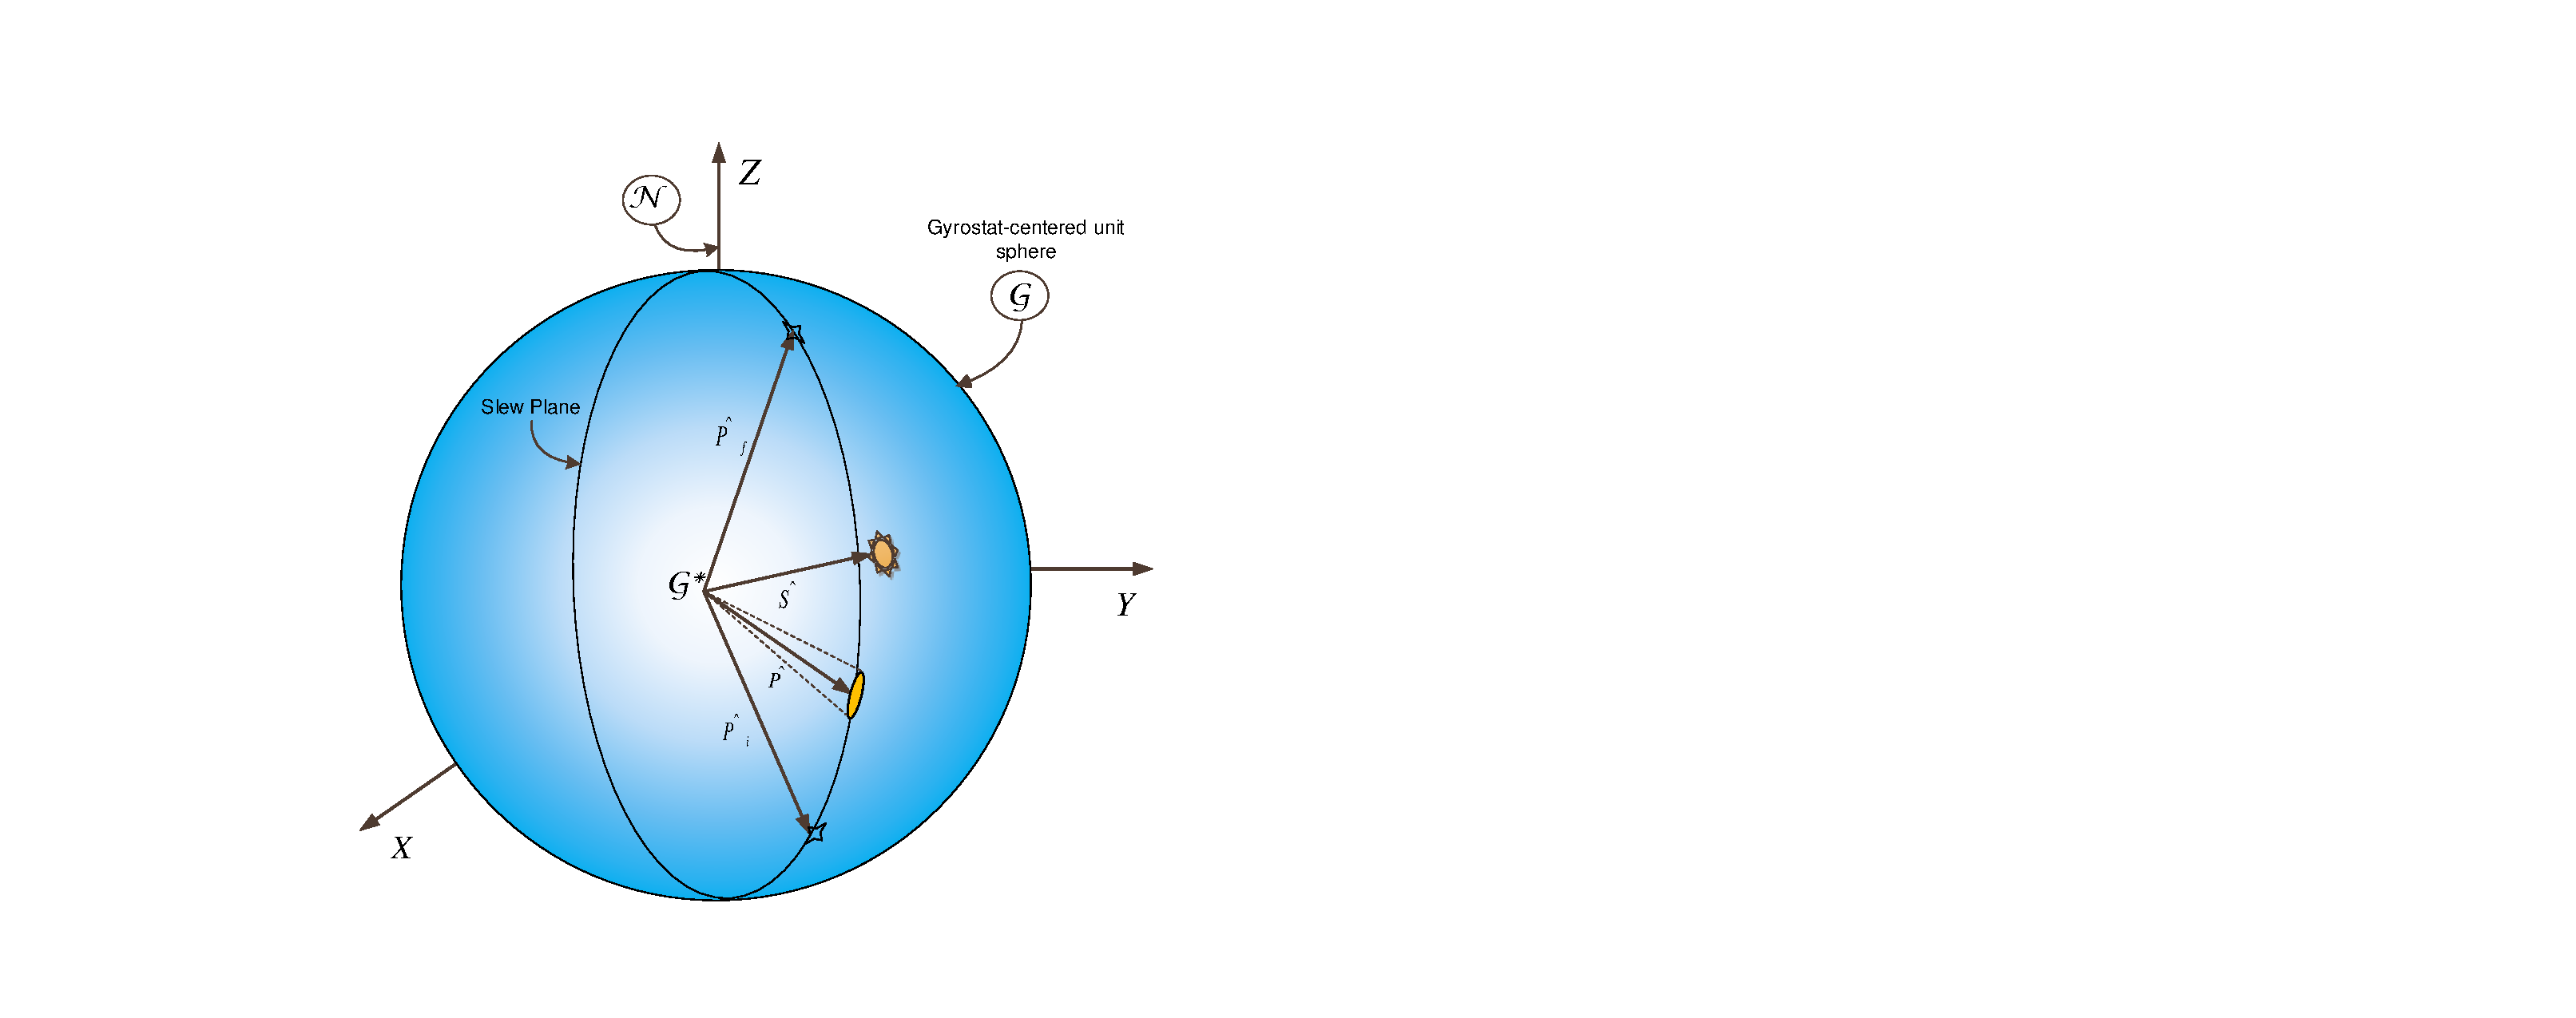
\includegraphics[width=3.5in]{./Figures/SASSchematic1}
				\caption{Gyrostat-centered unit sphere centered at point $\mathcal{G^*}$. }
			\end{center}
		\end{figure}

Throughout this paper, the left subscript of a vector denotes the reference frame in which the vector is expressed.		
\section{Sun-Avoidance Slew (SAS) Algorithm Description} 
	The first step is to determine if there is a sun vector intrusion. To this end, we check the angular separation, $\alpha$, between the sun unit vector, $_\mathcal{N}\hat{S}$, and the $\hat{P}_i-\hat{P}_f$ plane, or ``slew plane,''
		\begin{equation}
		\alpha=\frac{\pi}{2}-\cos^{-1}(\hat{S}\cdot\hat{e}),
		\end{equation}
		where the eigenaxis unit vector is determined by
		\begin{equation}\label{eaxis}
		\hat{e}=\frac{\hat{P}_i\times\hat{P}_f}{|\hat{P}_i\times \hat{P}_f|}.
		\end{equation} 
If $|\alpha|>=\epsilon_p$ then the sun vector intrusion has not happened. Otherwise, we need to perform the sun-avoidance slew maneuver which is explained in the next section.
	
%	\end{enumerate}
	
	%-------------------------------------------------------------------------------------------------------------------------------------------------------------------
	
	\subsubsection{Slew Planning}
	If $|\alpha|<\epsilon_p$, then we need to plan the sun-avoidance slew in the following steps: 
	\begin{enumerate}
		\item The $1^{st}$ slew is around the eigenaxis, $\hat{e}$, through angle $\phi_1$:
		%		\end{enumerate}
		\begin{equation}\label{phi1_1}
		\phi_1 = \cos^{-1}(\hat{P}_i\cdot_\mathcal{G}\hat{S}_{||})-\epsilon_p,\\
		\end{equation}
		\begin{figure}[H]
			\begin{center}
				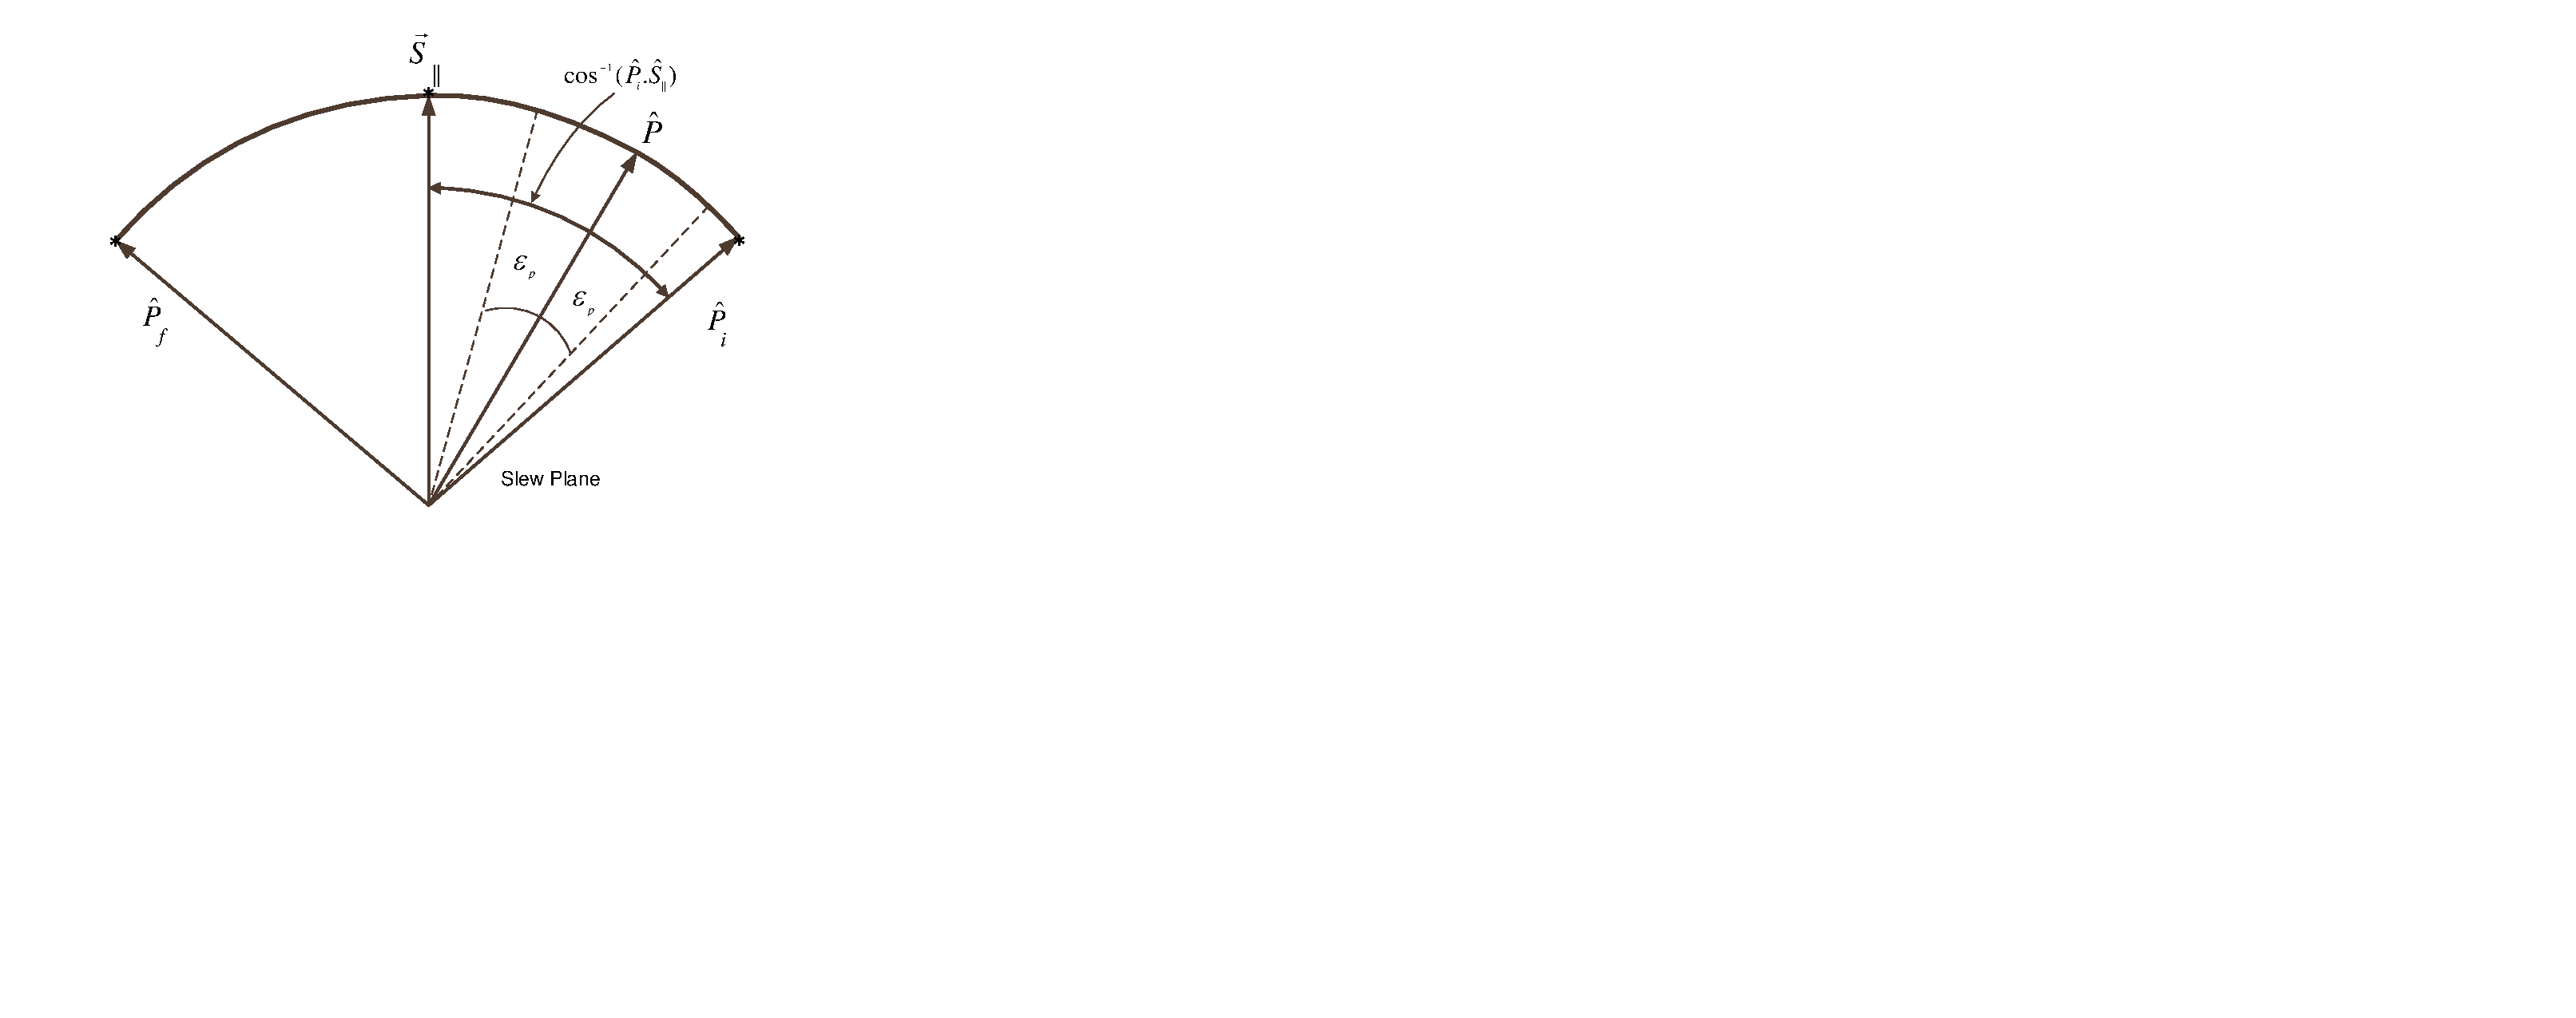
\includegraphics[width=3.5in]{./Figures/SVAS_1r_modified}
				\caption{View of the sensitive instrument's LOS vector motion during the $1^{st}$ slew from above the slew plane.}
			\end{center}
		\end{figure}
		\begin{figure}[h!]
			\centering
				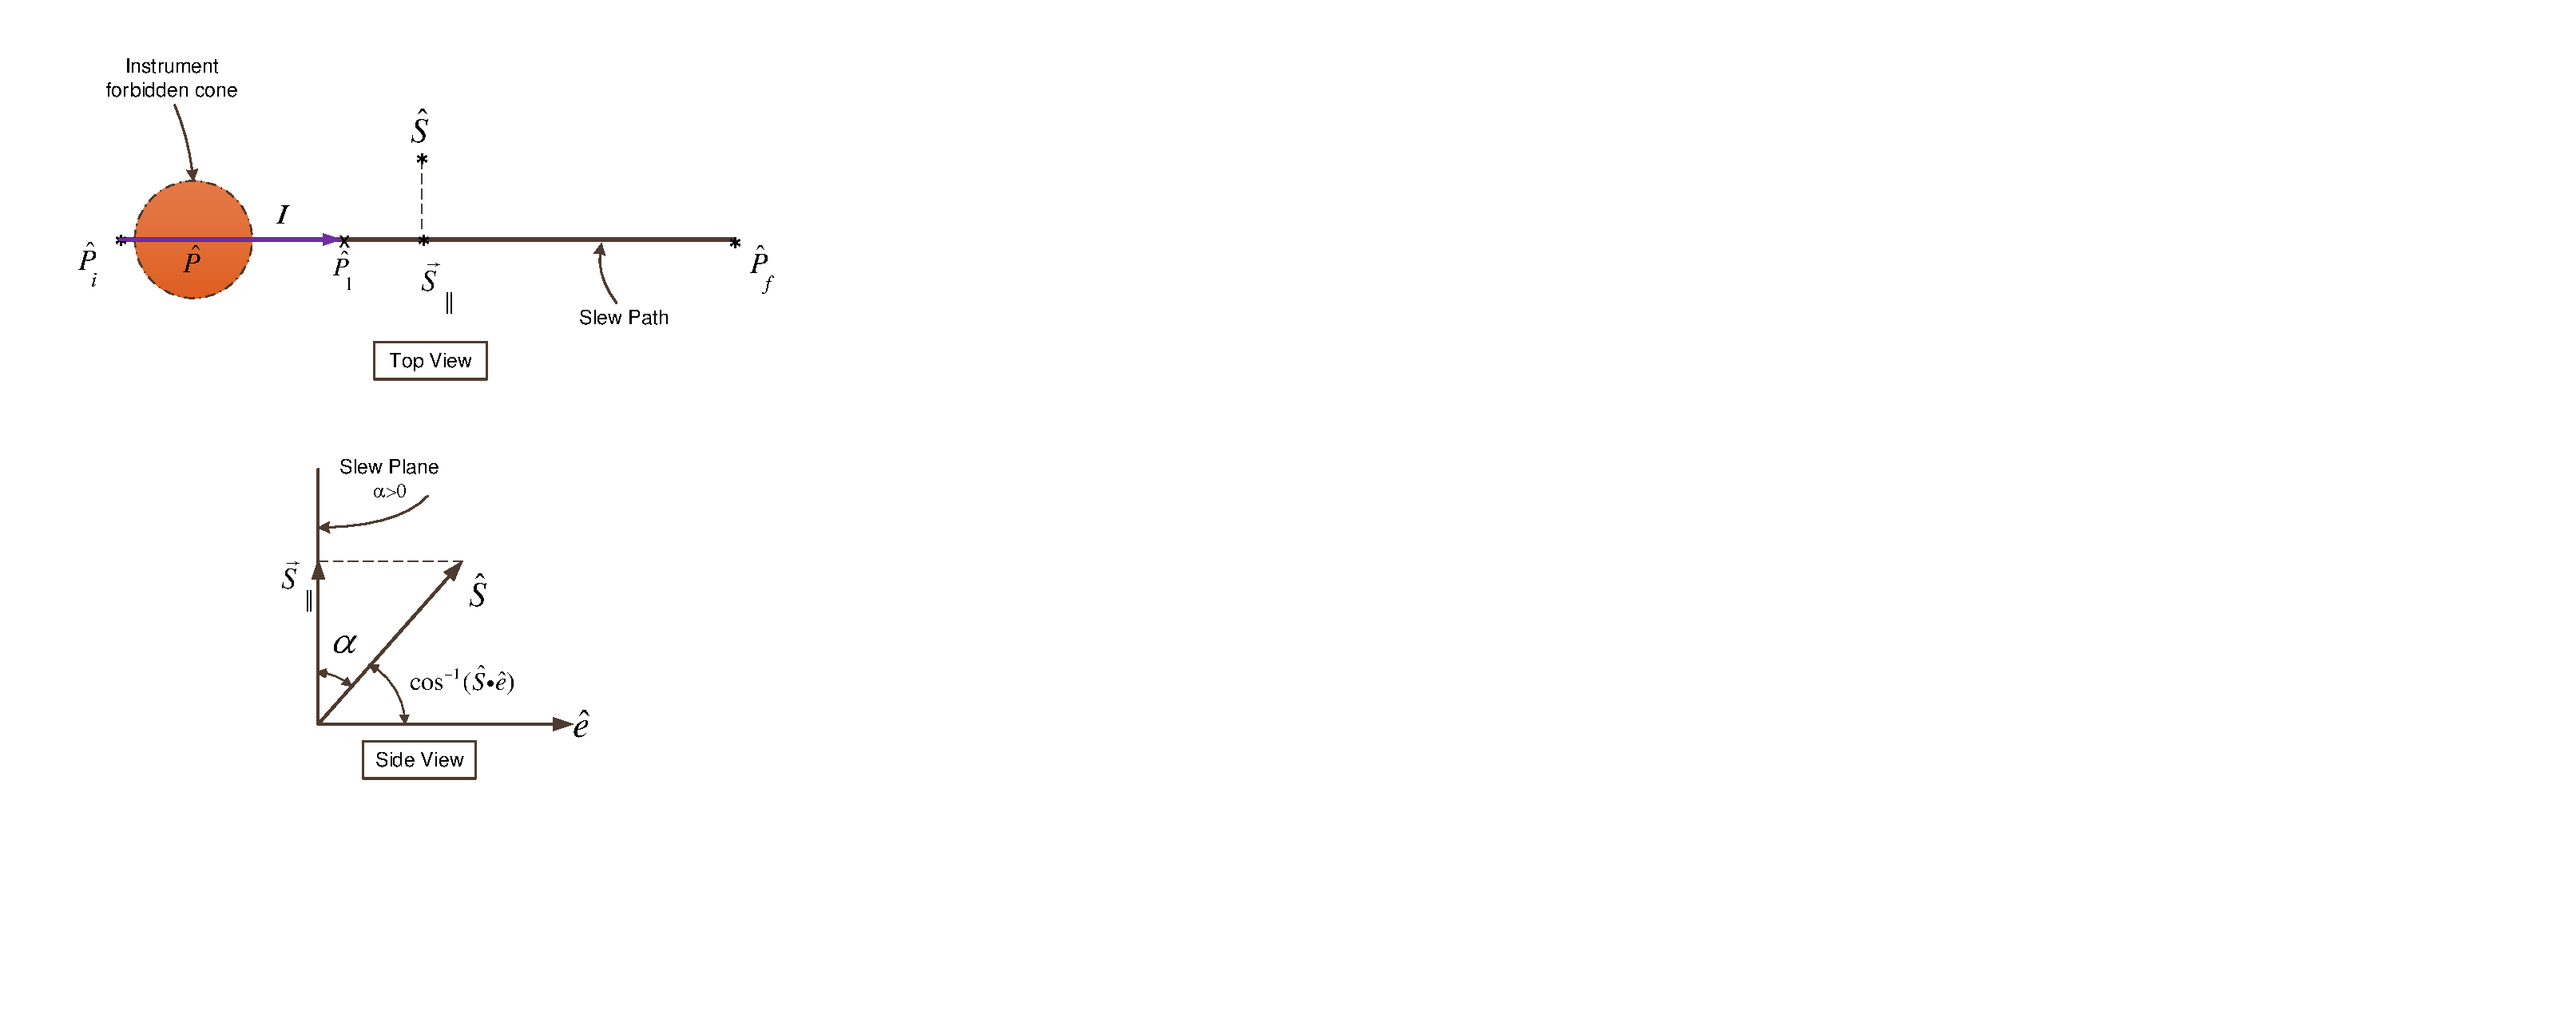
\includegraphics[width=3.5in]{./Figures/SVAS_1rb_modified}
				\caption{Top and side views of the sensitive instrument's LOS vector motion during the $1^{st}$ slew.}
		\end{figure}
		where 
		\begin{equation}\label{Sbar}
		\vec{S}_{||}=\hat{S}\cos\alpha, 
		\end{equation}
		and
		\begin{equation}\label{Shat}
		\hat{S}_{||}=\frac{\vec{S}}{|\vec{S}|}.
		\end{equation}
	
		It should be noted that the vector $\hat{S}_{||}$ is in the $\mathcal{N}$-frame. Therefore, it should be transformed in the $\mathcal{G}$-frame before it can be used in Eq. (\ref{phi1_1}). The vector $\hat{P}_1$ denotes the position vector of $\hat{P}$ at the end of $1^{st}$ slew.
		\item The $2^{nd}$ slew is around the unit sun vector, $\hat{S}$, can be found from the spherical triangle $\hat{P}_1\hat{S}\hat{P}_2$ shown in Fig.~\ref{sphericaltriangle}. The rotation angle $\phi_2$, from $\hat{P}_1$ to $\hat{P}_2$ around $\hat{S}$ is given by\cite{Wertz2011} 
		\begin{enumerate}
			\item when $\alpha\neq 0$
	\begin{equation}
	\phi_2=2\tan^{-1}\Big[ \frac{\hat{S}\cdot (\hat{P}_1\times\hat{S}_{||})}{(\hat{P}_1\cdot\hat{S}_{||})-(\hat{S}\cdot\hat{P}_1)(\hat{S}\cdot\hat{S}_{||})}\Big], 
	\end{equation}
or
	\begin{equation} 
	phi_2=2\tan^{-1}\Big[ \frac{\sin\alpha \sin\epsilon_p}{\cos\epsilon_p-\cos\theta\cos\alpha}\Big].
	\end{equation}
			\begin{figure}[h!]
				\centering
					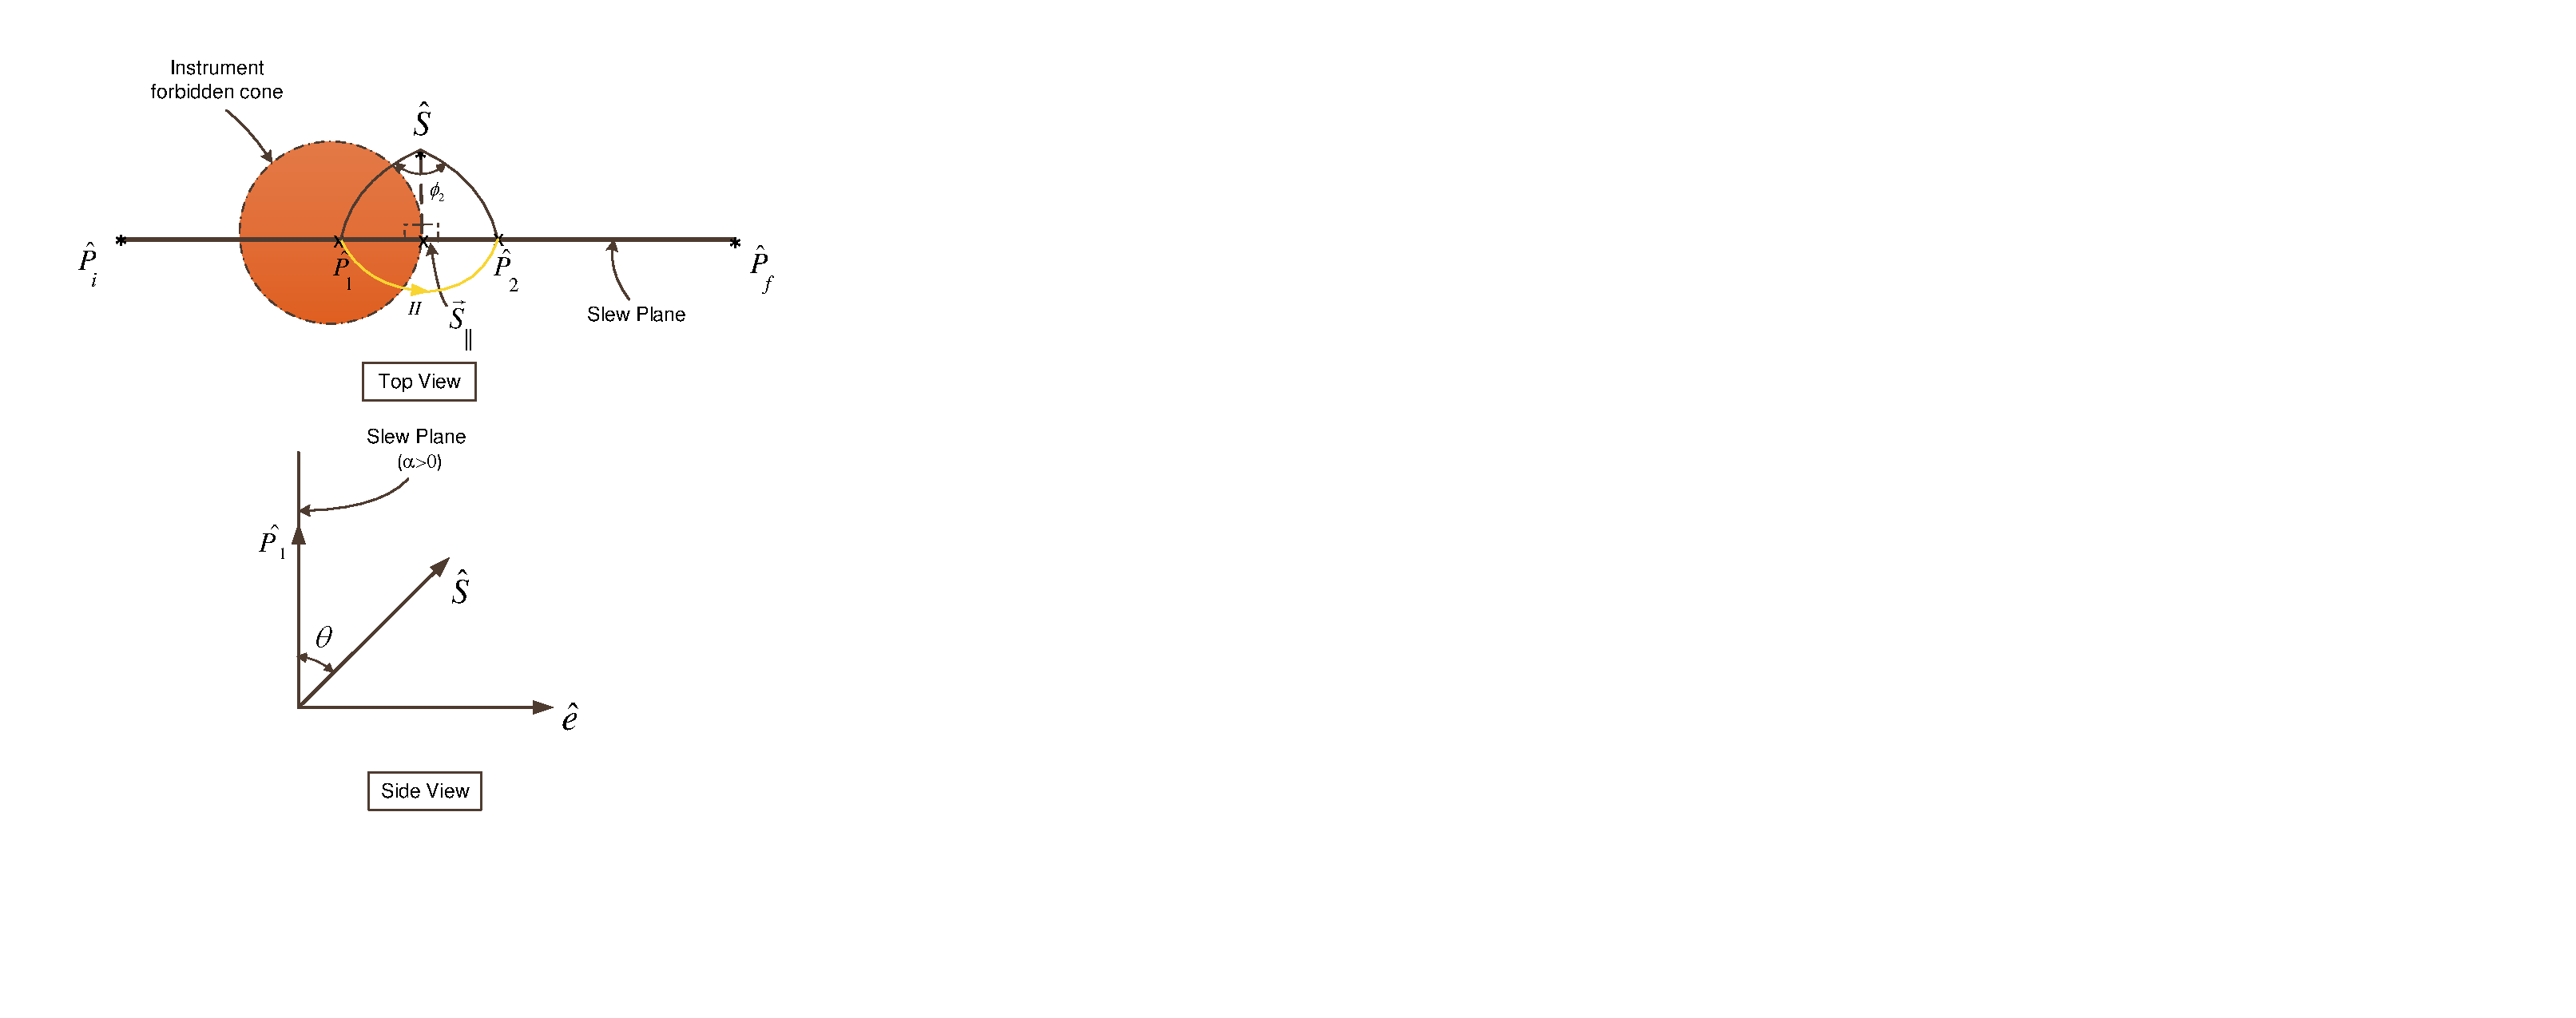
\includegraphics[width=3.25in]{./Figures/SVAS_2r_modified}
					\caption{The sensitive instrument's LOS vector motion during the $2^{nd}$ slew when $\alpha\neq 0$.}
					\label{sphericaltriangle}
			\end{figure}			
			\item when $\alpha=0$
			\begin{equation}
				\phi_2 = \pi.
			\end{equation}
			\begin{figure}[h!]
				\centering
					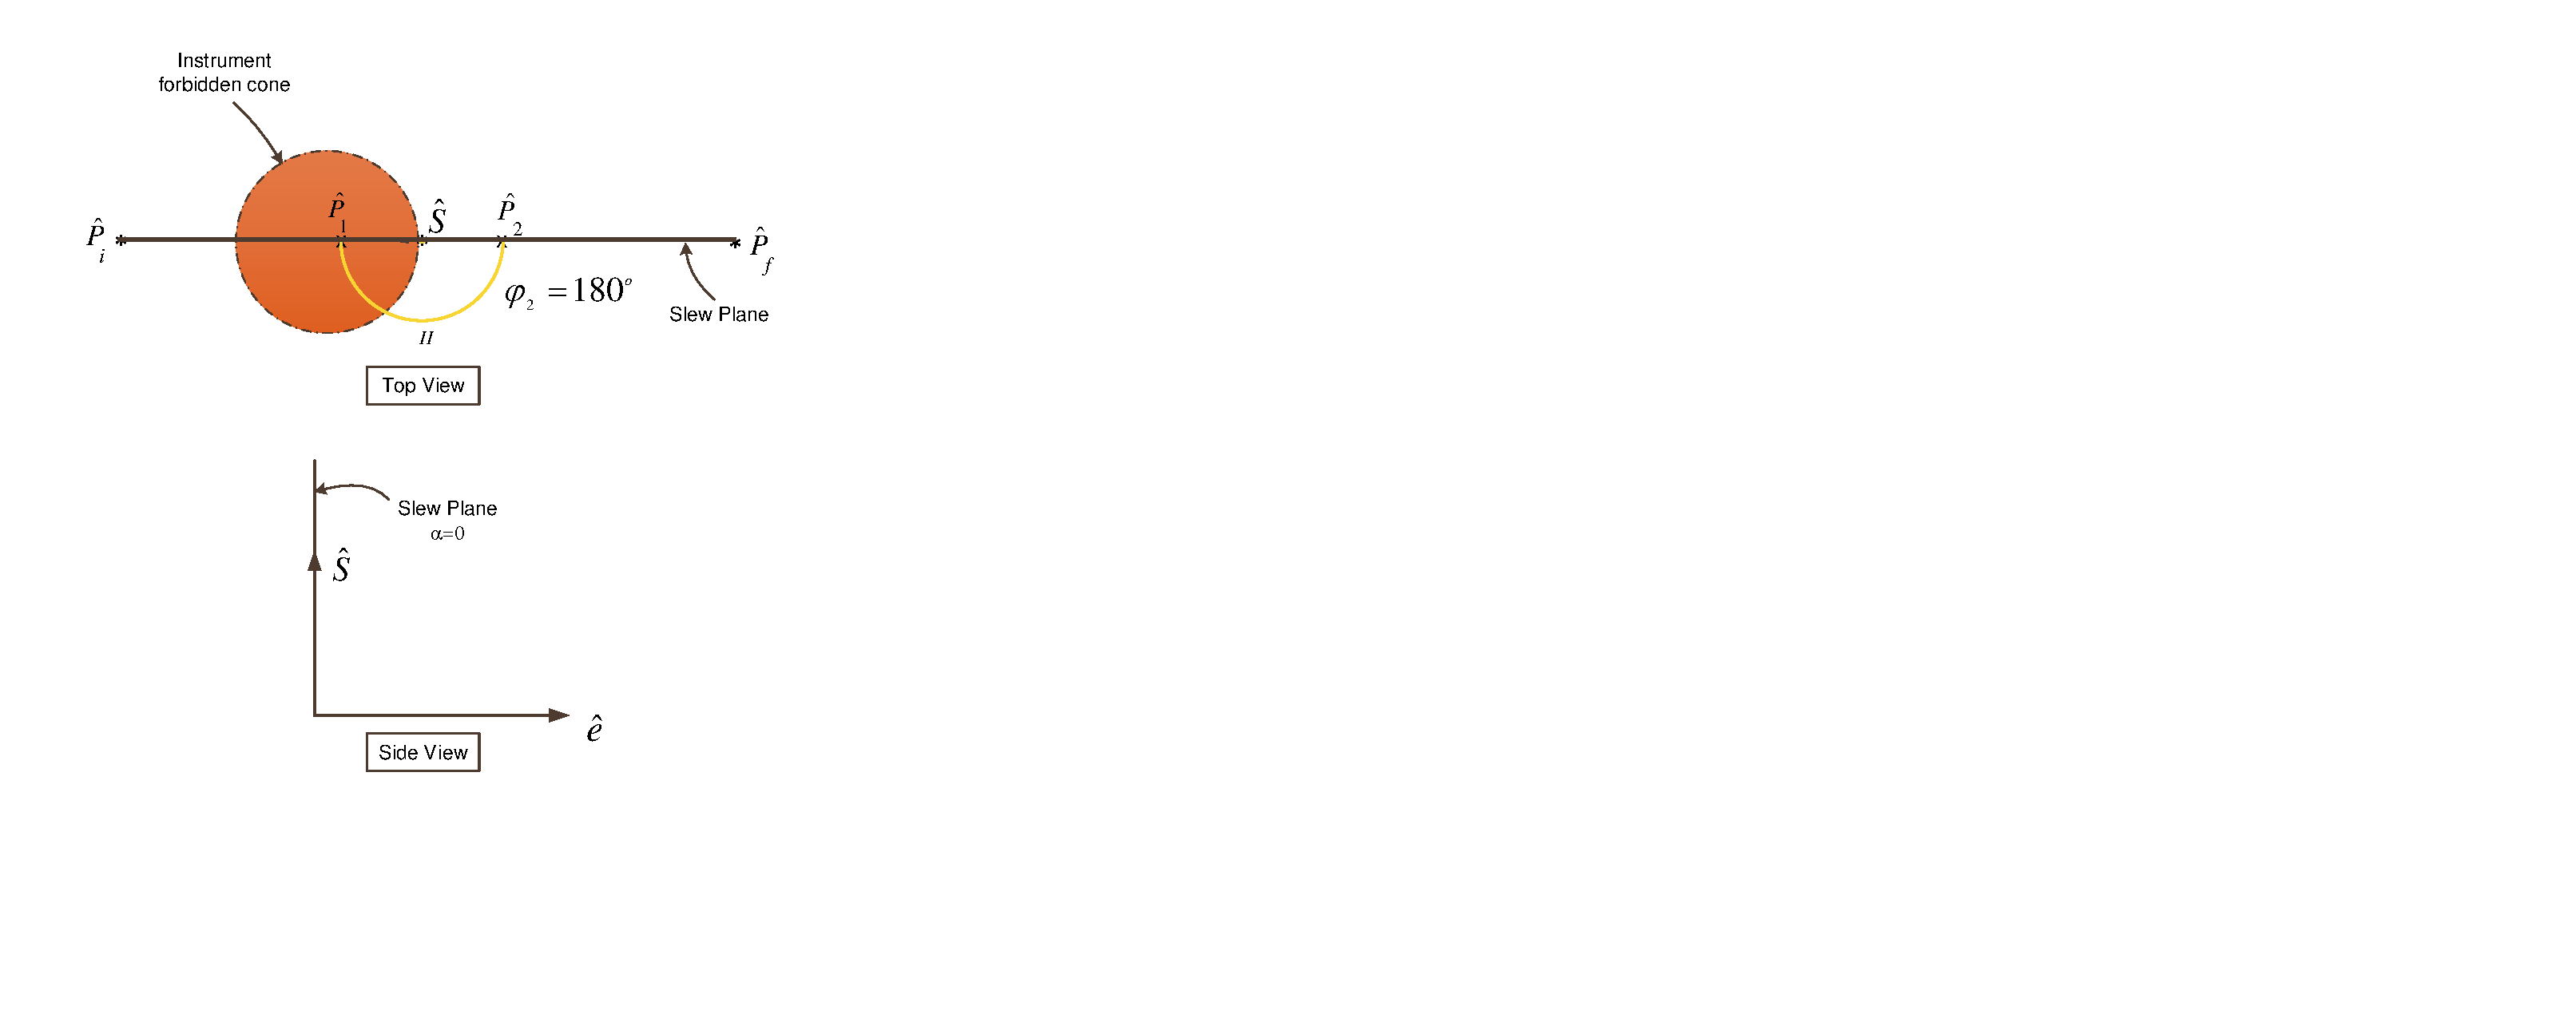
\includegraphics[width=3.5in]{./Figures/SVAS_3r_modified}
						\caption{The sensitive instrument's LOS vector motion during the $2^{nd}$ slew when $\alpha= 0$.}
			\end{figure}
		\end{enumerate}
		The vector $\hat{P}_2$ denotes the position vector of $\hat{P}$ at the end of $2^{nd}$ slew.
		%-------------------------------------------------------------------------------------------------------------------------------------------------------------------
		
		\item The $3^{rd}$ slew is about $\hat{e}$ through angle $\phi_3$:
		\begin{equation}\label{phi3_3}
		\phi_3 = \cos^{-1}(_\mathcal{G}\hat{P}_f\cdot\hat{S}_{||})-\epsilon_p.\\
		\end{equation}
		\begin{figure}[h!]
			\centering
				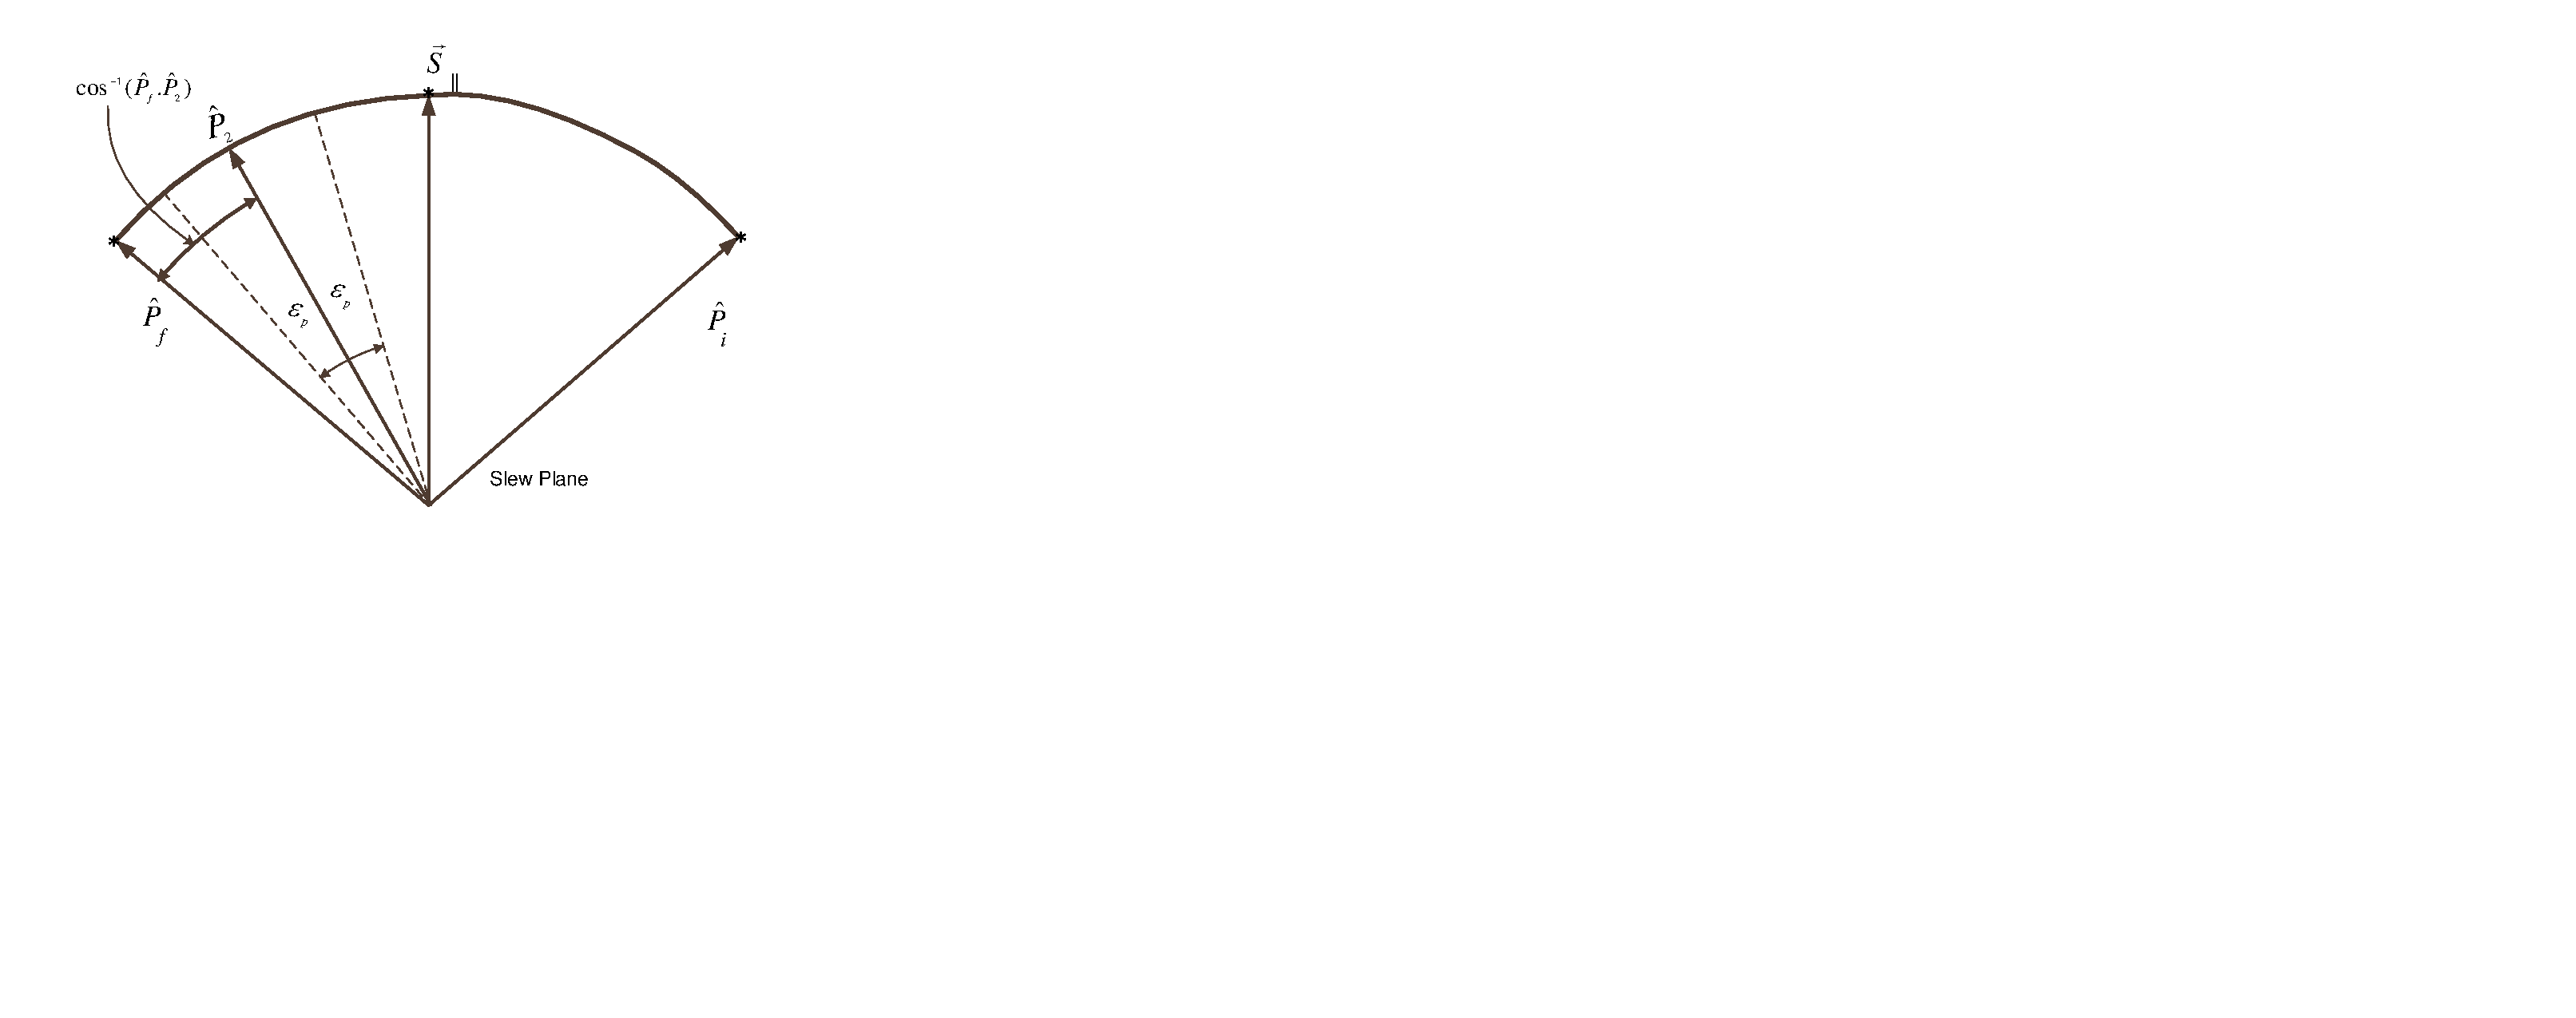
\includegraphics[width=3.5in]{./Figures/SVAS_4r}
					\caption{The sensitive instrument's LOS vector motion during the $3^{rd}$ slew.}
		\end{figure}
		%		\end{enumerate}
		%		\begin{enumerate}[4]
		Similar to the $1^{st}$ maneuver, the vector $_\mathcal{N}\hat{P}_f$ needs to be transformed to the $\mathcal{G}$-frame before doing the dot product in Eq. (\ref{phi3_3}). 
		\item The final slew about the instrument's LOS axis may be needed to go to the final attitude. 
	\end{enumerate}
	%	\end{enumerate}
	
	%-------------------------------------------------------------------------------------------------------------------------------------------------------------------
	
	\subsection{Summary of Algorithm} 	
	\begin{enumerate}
		\item Slew around the eigenaxis, $\hat{e}$, through angle $\phi_1$:		
		\begin{equation}\label{phi1}
		\phi_1 = \cos^{-1}(\hat{P}_i\cdot_\mathcal{G}\hat{S}_{||})-\epsilon_p.\\
		\end{equation}
		\item Slew around the $\hat{S}$ via:
		\begin{equation}\label{phi2}
		\phi_2=\left\{
		\begin{array}{ll}
		2\tan^{-1}\Big[ \frac{\sin\alpha \sin\epsilon_p}{\cos\epsilon_p-\cos\theta\cos\alpha}\Big],& when\  \alpha\neq 0\\
		\pi.& when\ \alpha=0\\
		\end{array}
		\right.
		\end{equation}
		\item Slew about $\hat{e}$ through angle:
		\begin{equation}\label{phi3}
		\phi_3 = \cos^{-1}(_\mathcal{G}\hat{P}_f\cdot\hat{S}_{||})-\epsilon_p.\\
		\end{equation}		
		\item If necessary, perform the final rotation, $\phi_4$, about the instrument's LOS axis to adjust the attitude. 
	\end{enumerate}
	
	%-------------------------------------------------------------------------------------------------------------------------------------------------------------------
	
	\begin{figure}[h!]
		\centering
		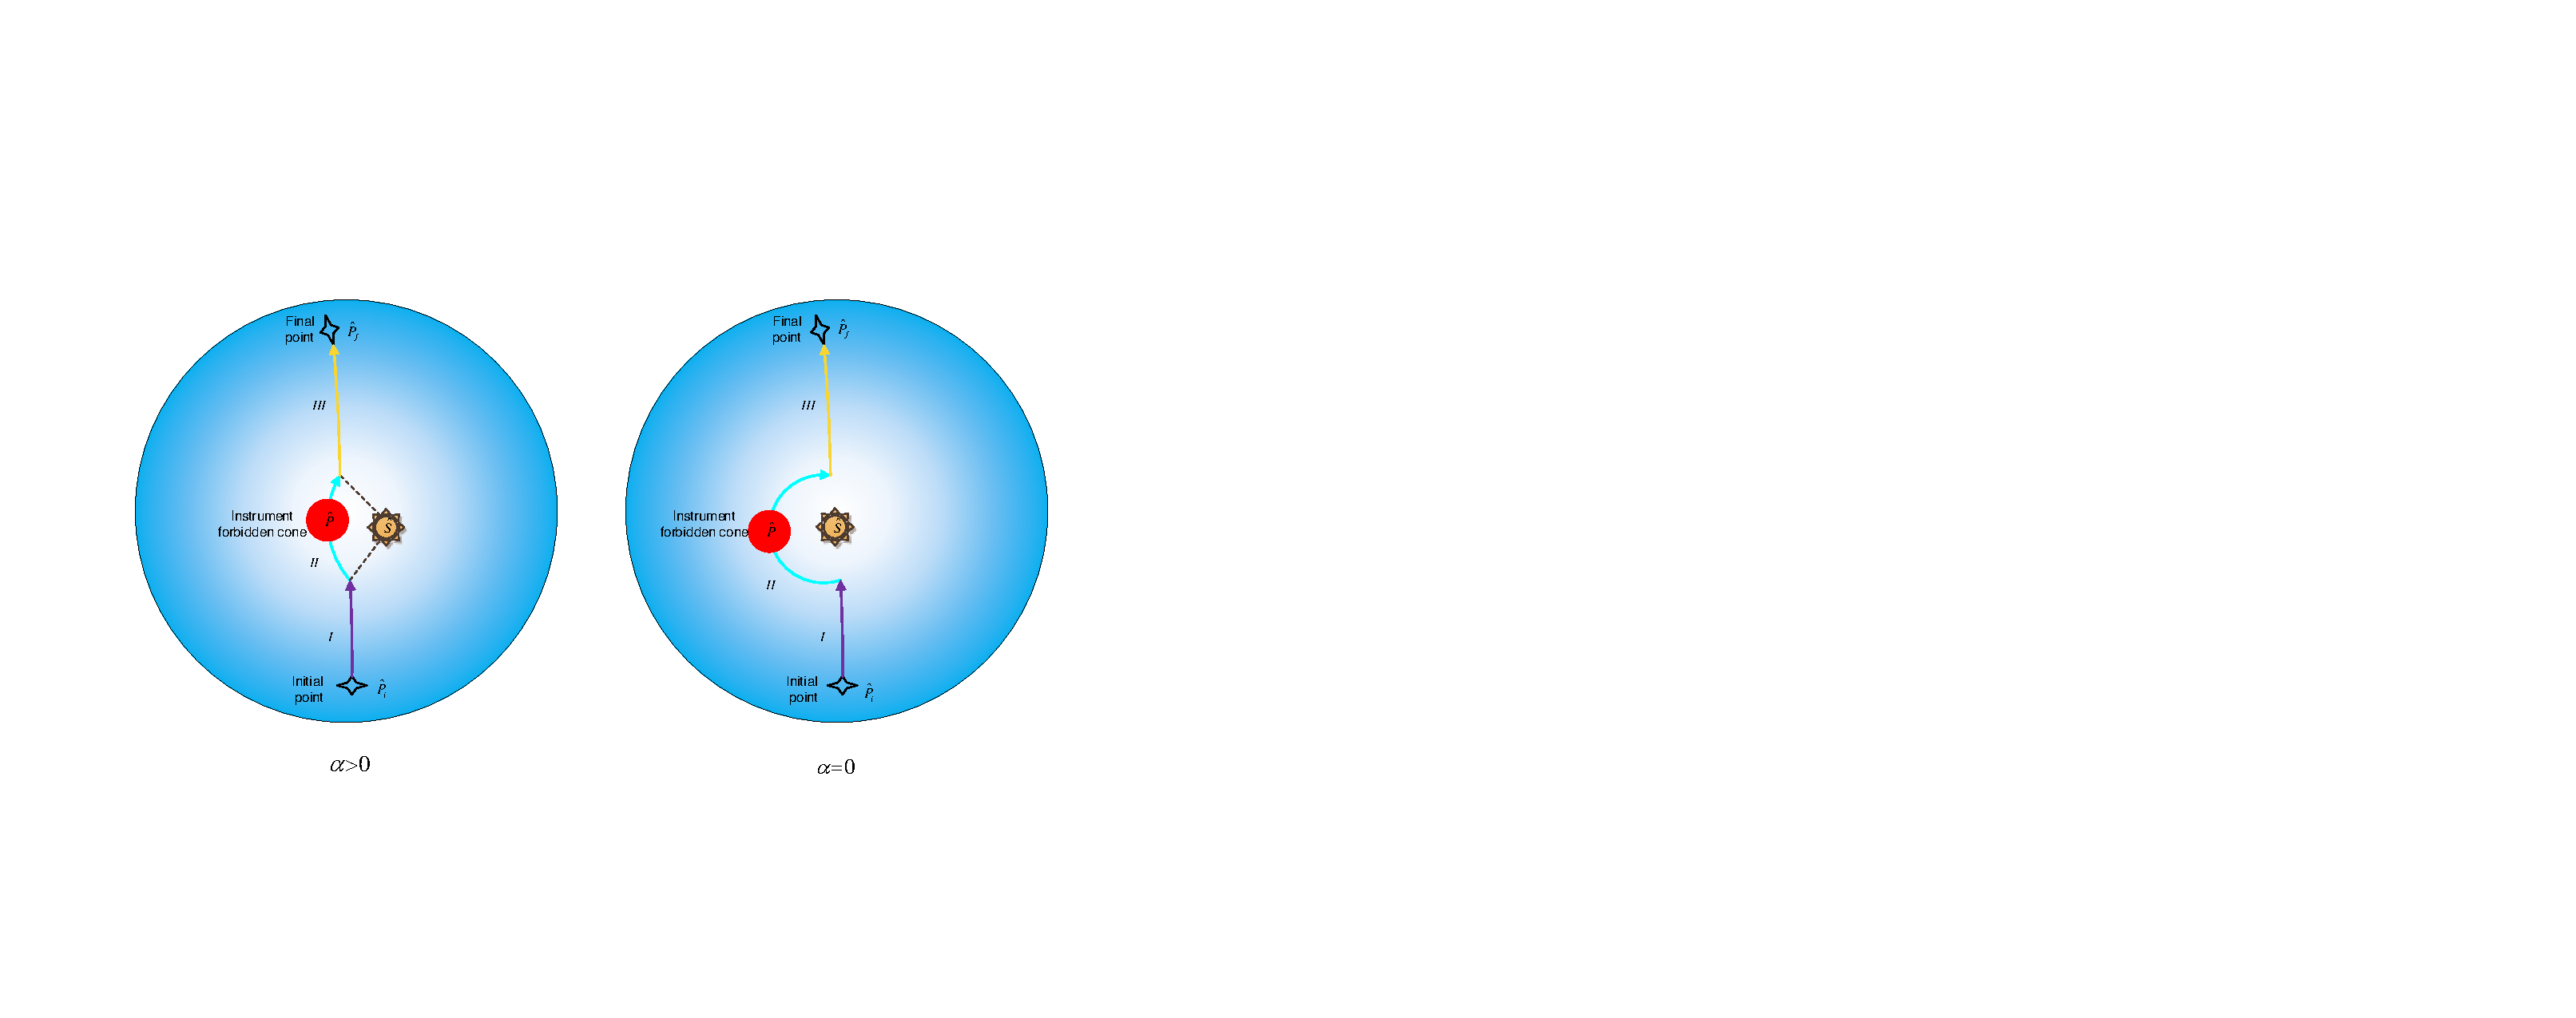
\includegraphics[width=6in]{./Figures/SASSchematic3}
		\caption{The trajectory of the instrument's LOS tip on the gyrostat-centered unit sphere during the SAS maneuver.}
	\end{figure}
	
	%-------------------------------------------------------------------------------------------------------------------------------------------------------------------
	
	\section{Slew Planning} 
	In this section we utilize the proposed sun-avoidance slew algorithm to generate the required angular rate, $_\mathcal{G}^\mathcal{N}\omega^\mathcal{T}(t)$, angular acceleration, $_\mathcal{G}^\mathcal{N}\dot{\omega}^\mathcal{T}(t)$, and quaternions, $^\mathcal{N}q^\mathcal{T}(t)$, for the control system. Fig. ~\ref{guidance_loop} shows how the generated commands are utilized by an attitude control system to guide the gyrostat in each leg of the SAS.
		\begin{figure}[h!]
		\centering
			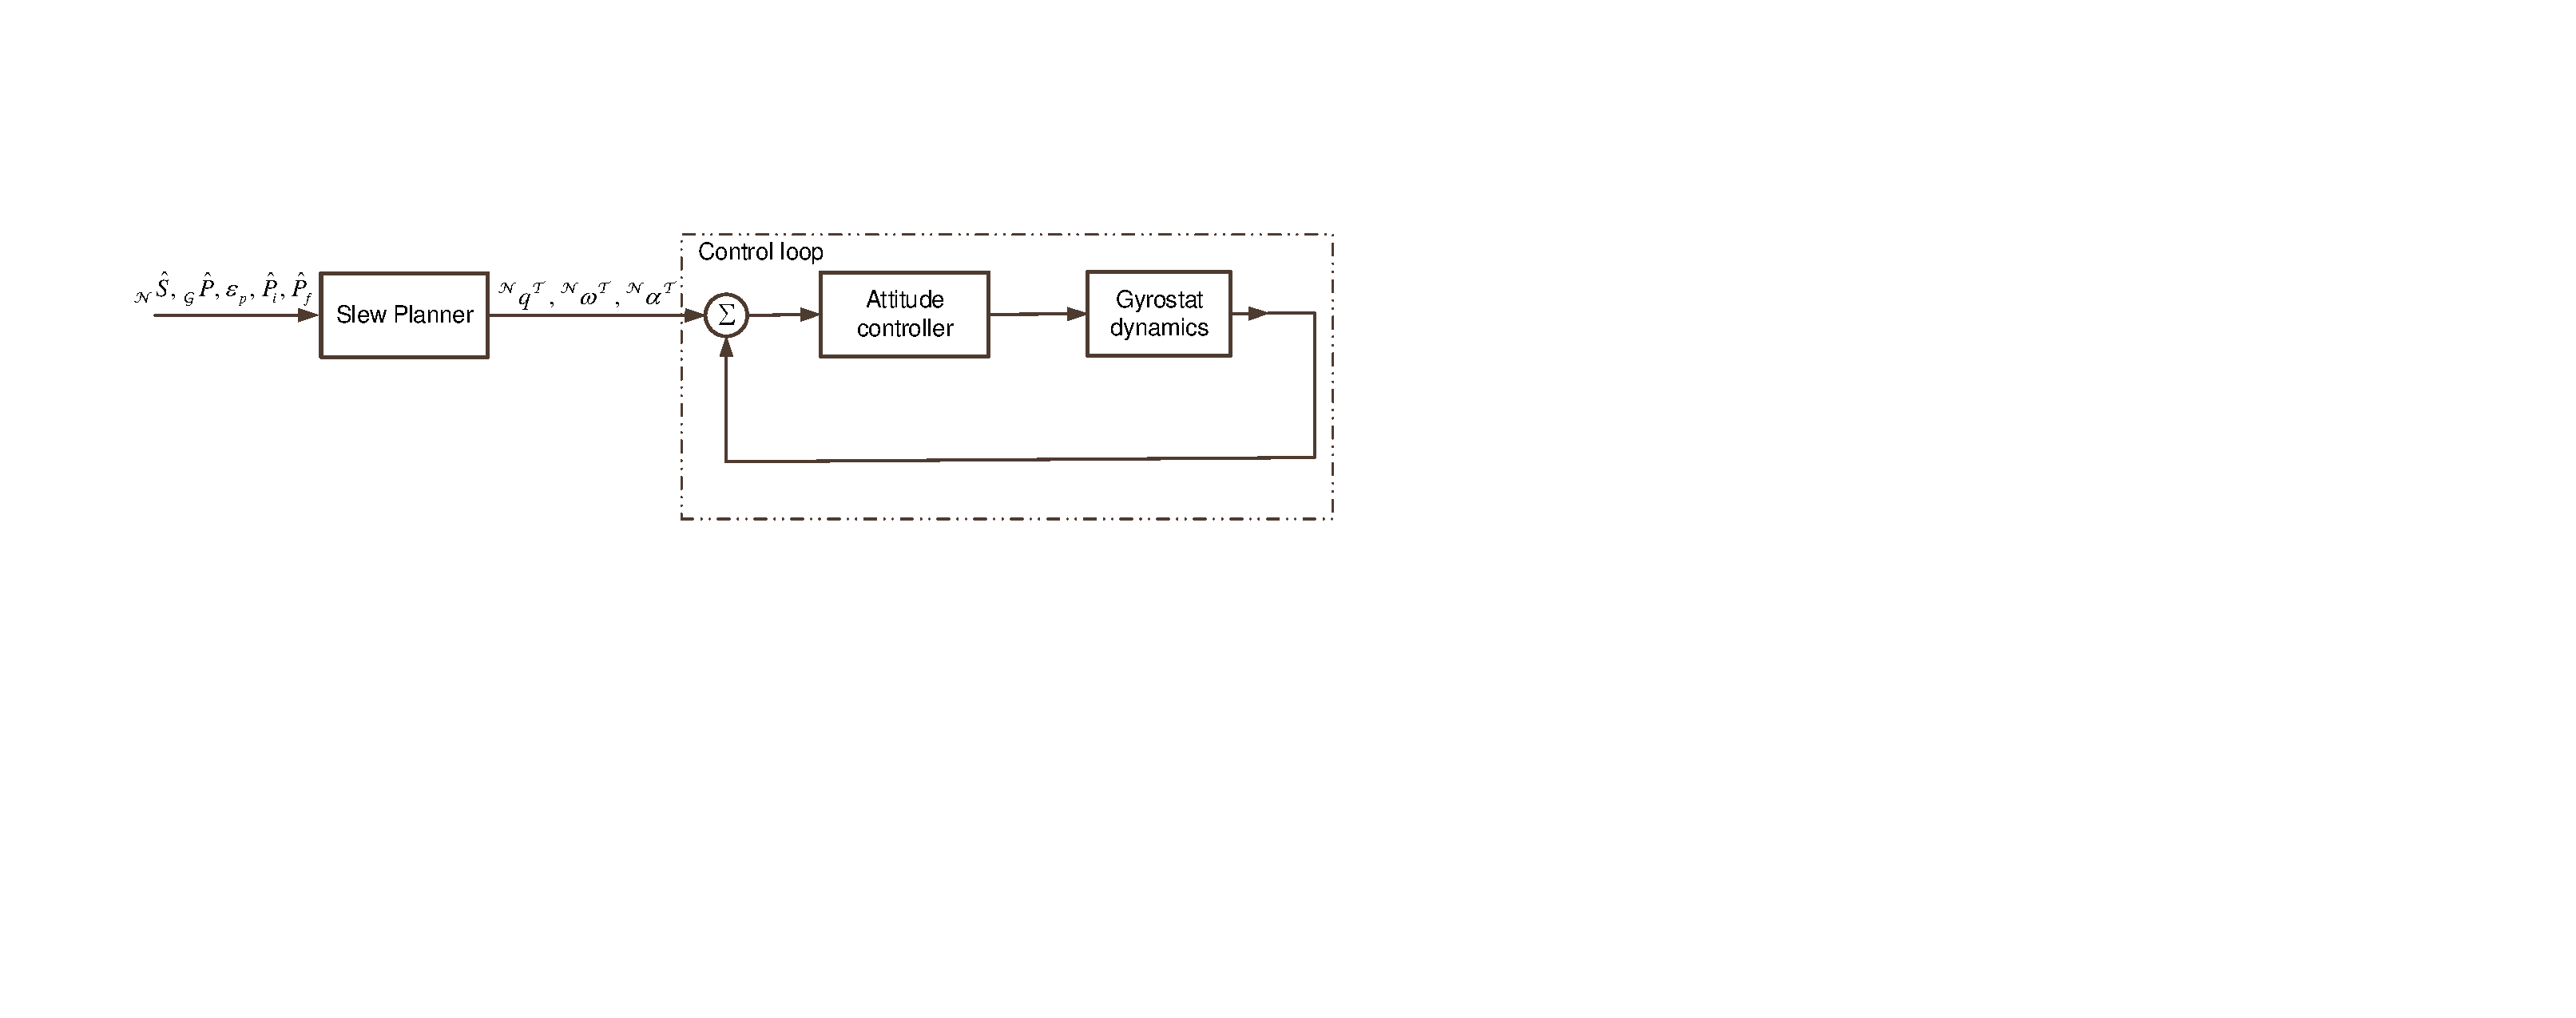
\includegraphics[width=4in]{./Figures/guidance_loop}  
			\caption{Block diagram of control loop. }
			\label{guidance_loop}
	\end{figure}	
	In the following, we formulate the problem of slew planning for two cases: 1) velocity and acceleration constraints and 2) acceleration constraint.
	\subsection{Case 1: Single-Axis, Agile Slew Maneuver with Velocity and Acceleration Constraints.}	 
	{\it Problem Statement}: Consider the motion of a gyrostat around a given inertially-fixed axis, $_\mathcal{N}\hat{e}$, as shown in Fig. ~\ref{s/c}. The problem of minimum-time slew maneuver around the $_\mathcal{N}\hat{e}$-axis can be formulated as:	
	\begin{equation}\label{costfunction}
	\underset{u\in \mathcal{U}}{Minimize}\ \mathcal{J}[x(.), u(.), t_f]=\int_{t0}^{t_f} dt,
	\end{equation}	
	subject to the following dynamic constraints:	
	\begin{equation}\label{system}
	\Sigma_\mathcal{G}:\left\{
	\begin{array}{l}
	\dot{x}_1=x_2, \\
	\dot{x}_2=M/I_{\hat{e}}^{\mathcal{G/G*}}=u, \\
	\end{array}
	\right.
	\end{equation}
	where the input $u$ is the acceleration, $\mathcal{U}$ is the set of all admissible controls, $x_1 \triangleq\phi$, $x_2=\dot{\phi}$, $M$ is the projection of the reaction wheels or other actuators' torque along $\hat{e}$, and $I_{\hat{e}}^{\mathcal{G/G*}}$ is the moment-of-inertia of gyrostat with respect to its center-of-mass along $\hat{e}$-axis. 
%	\begin{equation}
%	I_{\hat{e}}^{\mathcal{G/G*}}=\hat{e\ }I^{\mathcal{G/G*}}\ \hat{e}^T.
%	\end{equation}
	
	\begin{figure}[h!]
		\centering
			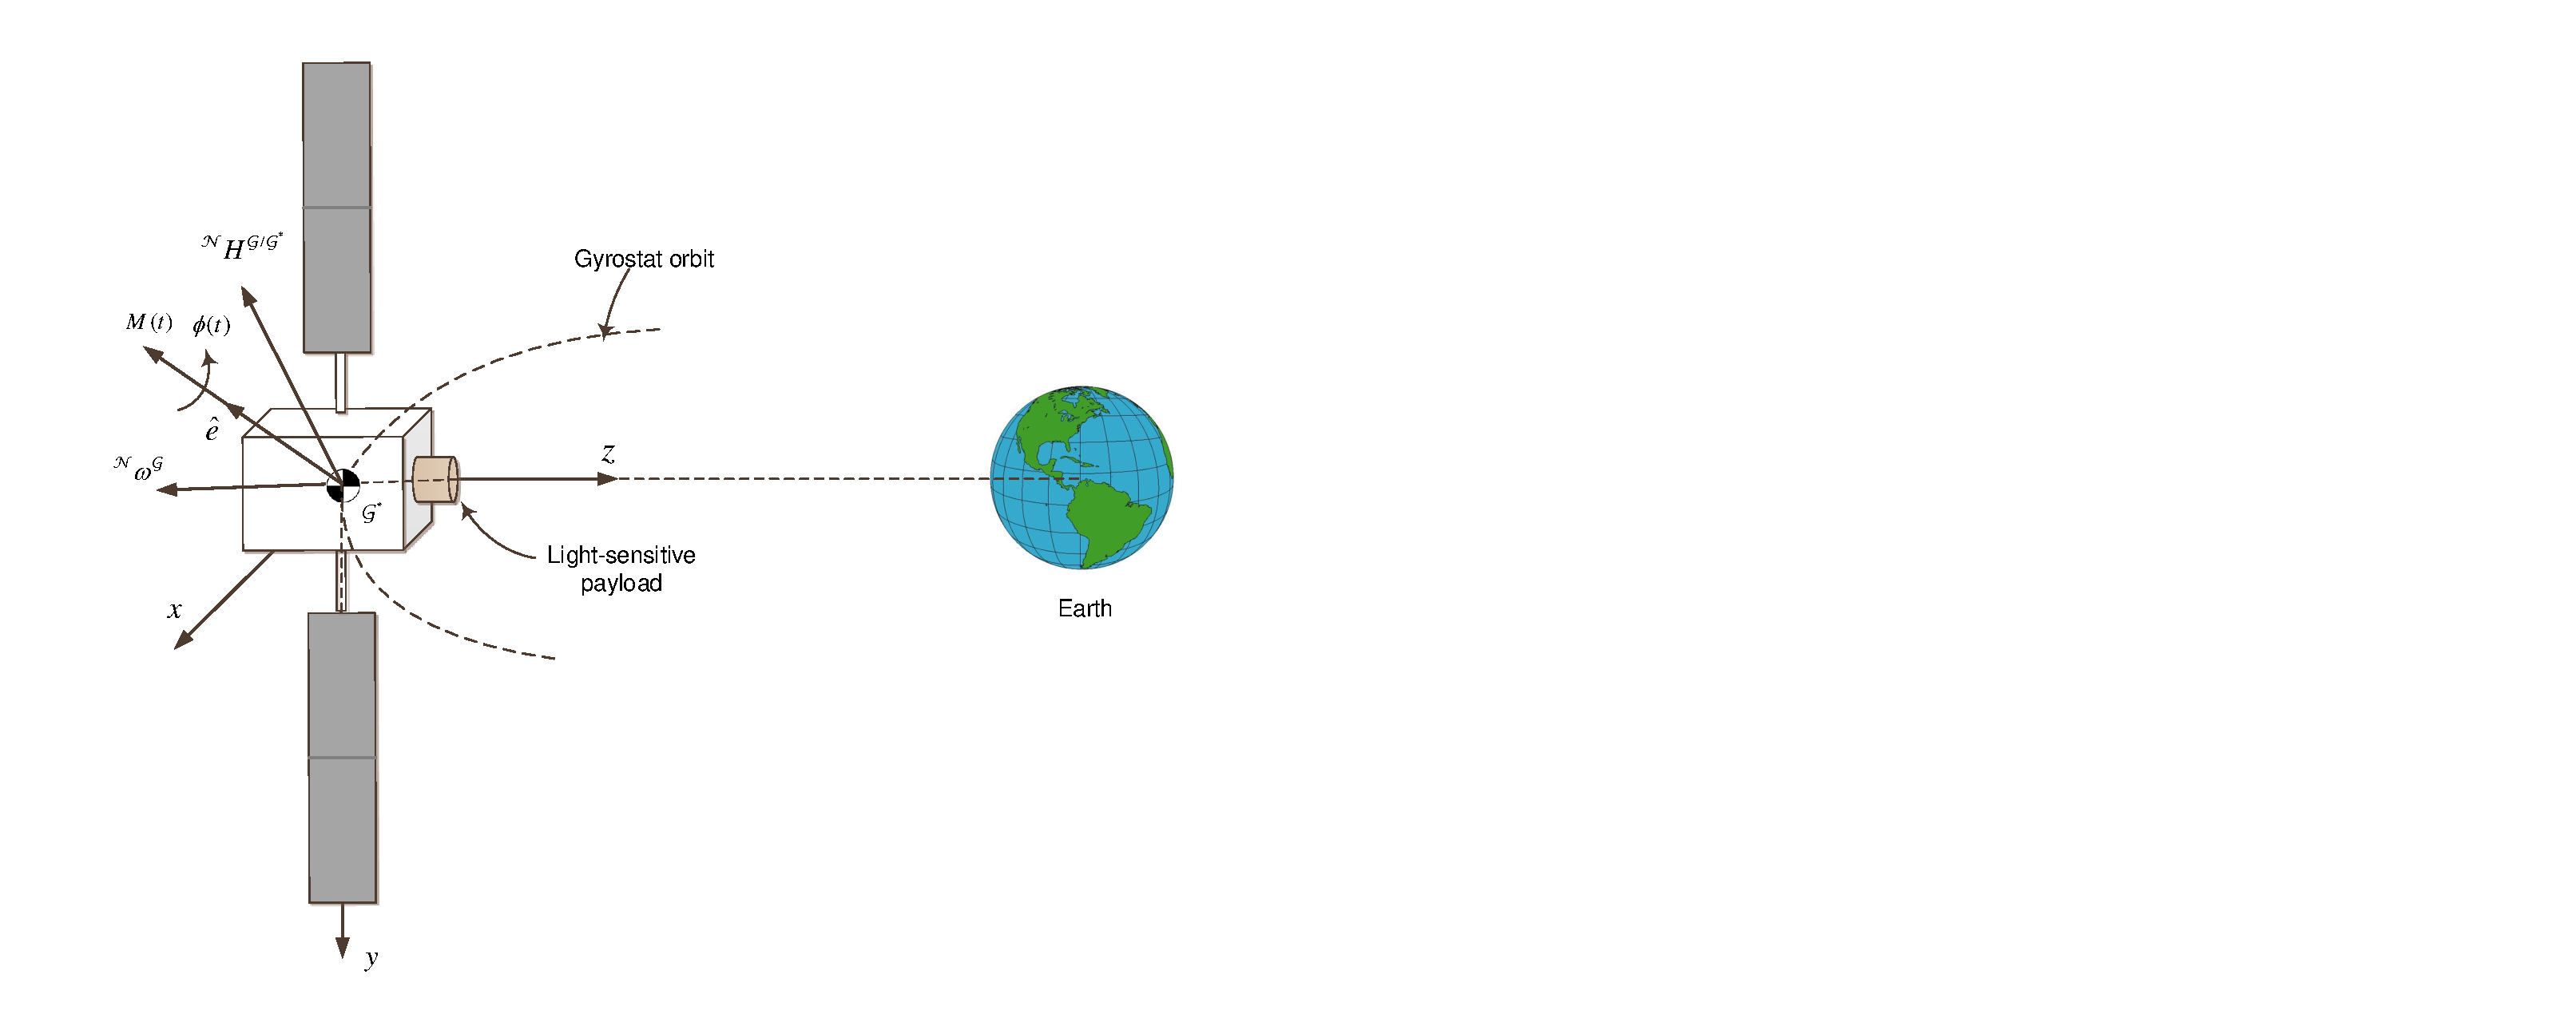
\includegraphics[width=4in]{./Figures/Spacecraft_earth}  
			\caption{A gyrostat rotating about the eigenaxis, $\hat{e}$.}
			\label{s/c}
	\end{figure}
	
	%-------------------------------------------------------------------------------------------------------------------------------------------------------------------

	where $T$ denotes transpose. The boundary conditions are given by
	\begin{equation}\label{Bcs}
	BCs:\left\{
	\begin{array}{l}
	\phi(t_0)=0, \phi(t_f)=\phi_{f},\\
	\dot{\phi}(t_0)=\dot{\phi}_{0},\dot{ \phi}(t_f)=\dot{\phi}_{f}, \\
	\end{array}
	\right.
	\end{equation}
	and the reaction wheels' angular momentum and control torque constraints can be transformed into the angular velocity and angular acceleration constraints as follows
	\begin{equation}\label{constraints1}
	C_1:\left\{
	\begin{array}{l}
	|x_2=\dot{\phi}|\leq \dot{\phi}_{max},\\
	|u=\ddot{\phi}|\leq \ddot{\phi}_{max},\\
	\end{array}
	\right.
	\end{equation}
	%in which 
	%\begin{equation}
	%\dot{\phi}_{max}=[I^{w/w^*}]^{-1}[^\mathcal{N}H^{\mathcal{G}/\mathcal{G*}}-(I^{\mathcal{G}/\mathcal{G}*}+I^{w/w*})^\mathcal{N}\omega^\mathcal{G}]/(e_x+e_y+e_z),
	%\end{equation}
	
	%-------------------------------------------------------------------------------------------------------------------------------------------------------------------
	
	%and
	%\begin{equation}\label{phiddotmax}
	%\ddot{\phi}_{max}= M_{max}/I_{\hat{e}}^{\mathcal{G/G*}},
	%\end{equation}	
	
Our objective is to find $^\mathcal{N}\omega^\mathcal{T}(t)$, $^\mathcal{N}\dot{\omega}^\mathcal{T}(t)$, and $^\mathcal{N}q^\mathcal{T}(t)$.\\
	
	%-------------------------------------------------------------------------------------------------------------------------------------------------------------------
	
	Using the optimal control theory and Pontryagin's minimum principle (PMP), we derive the necessary conditions for the optimal solution as follows:
	\begin{enumerate}
		\item State Eqs.:
		\begin{equation}
		\left\{
		\begin{array}{l}
		\dot{x}_1=x_2, \\
		\dot{x}_2=u, \\
		\dot{x}_3=(x_2+\dot{\phi}_{max})^2\mathbb{U}(-x_2-\dot{\phi}_{max})+(\dot{\phi}_{max}-x_2)^2\mathbb{U}(x_2-\dot{\phi}_{max}),
		\end{array}
		\right.
		\end{equation}
		where the unit step function, $\mathbb{U}$, is defined as
		\begin{equation}
		\mathbb{U}(X)=\left\{
		\begin{array}{l}
		1,   X>0, \\
		0,   X\leq 0.
		\end{array}
		\right.
		\end{equation}
		Note:  ($x_3(t_0)=x_3(t_f)=0$ \& $x_3(t)\geq 0$ ) $\rightarrow x_3(t)=0, t\in[t_0, t_f]$. 
		%				Note:  ($x_3(t_0)=x_3(t_f)=0$ \& $x_3(t)\geq 0$ ) $\rightarrow x_3(t)=0, \foral t\in[t_0, t_f]. $  
		
		\item Hamiltonian:
		\begin{equation}
		\begin{split}
		\mathscr{H}=& 1+\lambda_1x_2+\lambda_2u+\lambda_3\Big[(x_2+\dot{\phi}_{max})^2\mathbb{U}(-x_2-\dot{\phi}_{max})\\
		& +(\dot{\phi}_{max}-x_2)^2\mathbb{U}(x_2-\dot{\phi}_{max})\Big].
		\end{split}
		\end{equation}
		%			\end{enumerate}
		
		%-------------------------------------------------------------------------------------------------------------------------------------------------------------------
		
		%			\begin{enumerate}
		%				\conti
		%				\small{
		\item Costate Eqs.:
		\begin{equation}
		\left\{\begin{array}{l}
		\dot{\lambda}_1=-\frac{\partial{\mathscr{H}}}{\partial{x_1}}=0,\\
		\dot{\lambda}_2=-\frac{\partial{\mathscr{H}}}{\partial{x_2}}=-\lambda_1-2\lambda_3(x_2+\dot{\phi}_{max})\mathbb{U}(-x_2-\dot{\phi}_{max})\\
		+2\lambda_3(\dot{\phi}_{max}-x_2)\mathbb{U}(x_2-\dot{\phi}_{max}),\\
		\dot{\lambda}_3=-\frac{\partial{\mathscr{H}}}{\partial{x_3}}=0.\\
		\end{array}
		\right.
		\end{equation}
		\item Applying the Pontryagin's minimum principle (PMP),
		\begin{equation}
		u^*=arg \underset{u\in\mathcal{U}}{min} \mathscr{H},
		\end{equation}
		where $\mathcal{U}$ defines the domain of feasible controls. The optimal control can be determined as
		\begin{equation}
		u^*(t)=\left\{
		\begin{array}{ll}
		\ddot{\phi}_{max}&\lambda_2<0,\\
		?& \lambda_2=0,\\
		-\ddot{\phi}_{max}&\lambda_2>0.
		\end{array}
		\right.
		\end{equation}
		%				}
		%			\end{enumerate}
		%			\seti
		This is a {\it singular arc} optimal control problem.
		
		%-------------------------------------------------------------------------------------------------------------------------------------------------------------------
		
		\item Determining the optimal control in the singular arc:
		\begin{equation}
		\frac{d^2}{dt^2}\Big(\frac{\partial \mathscr{H}}{\partial u}\Big)=\ddot{\lambda}_2=0\rightarrow \dot{x}_2=0\rightarrow u^*=0.
		\end{equation}
		\item Checking the Generalized Legendre-Clebsch condition for optimality:
		\begin{equation}
		(-1)^2\frac{\partial}{\partial u}\Big[\frac{d^2}{dt^2}\Big(\frac{\partial \mathscr{H}}{\partial u}\Big)\Big]=1\geq 0.
		\end{equation}
		\item Checking the transversality condition:
		\begin{equation}
		\mathscr{H}|_{(*,t_f)}=0\  \text{and} \ \mathscr{H}\neq\mathscr{H}(t)\rightarrow \mathscr{H}=0, \forall t\in[t_0, t_f].
		\end{equation}
	\end{enumerate}
	%	\seti
	
	%-------------------------------------------------------------------------------------------------------------------------------------------------------------------
	The angular acceleration profile is bang-off-bang, as shown in Fig. ~\ref{bang_off_bang}
	\begin{equation}\label{phidd_cons}
	u^*(t)=\ddot{\phi}(t)=\left\{
	\begin{array}{ll}
	\ddot{\phi}_{max}& when\  t_0\leq t\leq t_1,\\
	0& when\  t_1\leq t \leq t_2,\\
	-\ddot{\phi}_{max}& when \ t_2\leq t\leq t_f.
	\end{array}
	\right.
	\end{equation}

	\begin{figure}[h!]
	\centering
	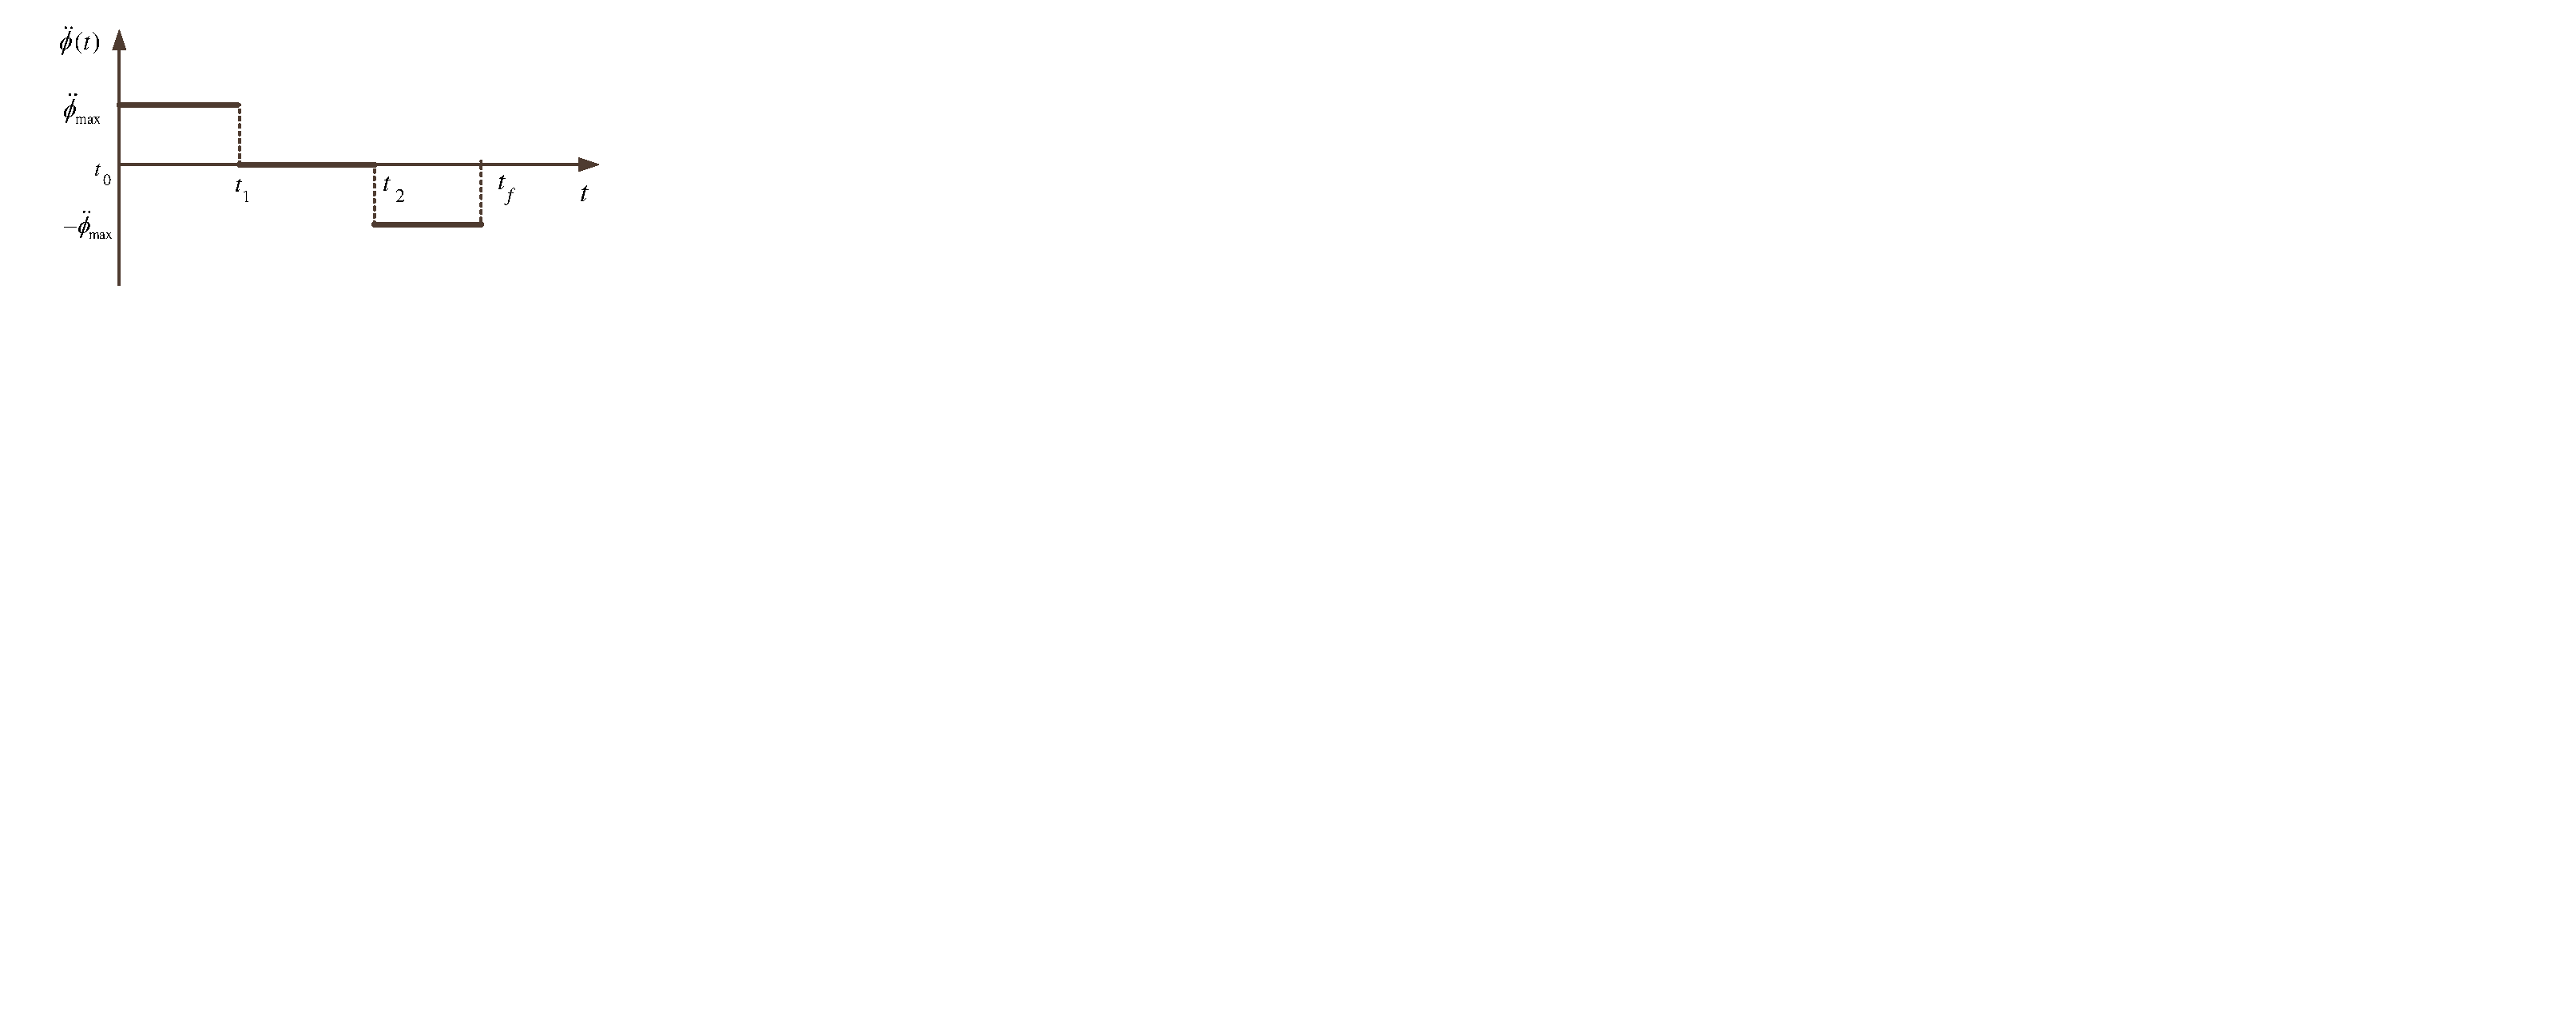
\includegraphics[width=3.5in]{./Figures/bang_off_bang}
	\caption{The optimal control law for case 1.}
	\label{bang_off_bang}
	\end{figure}
 The angular velocity profile can be determined as

	\begin{equation}\label{phid_cons}
	\dot{\phi}(t)=\left\{
	\begin{array}{ll}
	\dot{\phi}_0+\ddot{\phi}_{max}(t-t_0)& when\  t_0\leq t\leq t_1,\\
	\dot{\phi}_{max}& when\  t_1\leq t \leq t_2,\\
	\dot{\phi}_{max}-\ddot{\phi}_{max}(t-t_2)& when \ t_2\leq t\leq t_f.
	\end{array}
	\right.
	\end{equation}

and the angular position can be find by direct integration of Eq. (\ref{phid_cons}),
	\begin{equation}\label{phi_cons}
	\phi(t)=\left\{
	\begin{array}{ll}
	\dot{\phi}_0(t-t_0)+\frac{1}{2}\ddot{\phi}_{max}(t-t_0)^2& when\  t_0\leq t\leq t_1,\\
	\phi(t_1)+ \dot{\phi}_{max}(t-t_1)& when\  t_1\leq t \leq t_2,\\
	\phi(t_2)+\dot{\phi}_{max}(t-t_2)-\frac{1}{2}\ddot{\phi}_{max}(t-t_2)^2& when \ t_2\leq t\leq t_f.
	\end{array}
	\right.
	\end{equation}
	
%-------------------------------------------------------------------------------------------------------------------------------------------------------------------

Using the conditions, $\dot{\phi}(t_1)=\dot{\phi}_{max}$, $\dot{\phi}(t_f)=\dot{\phi}_f$, $\phi(t_f)=\phi_f$, we can determine switching times $t_1$, $t_2$, and final time $t_f$. Depending on the size of $\phi$ and the maximum velocity and acceleration constraints, the gyrostat may or may not reach its maximum allowed velocity during a slew, which in turn determines the calculation of switching times. There is a threshold angle, which is called $\phi_t$ and is calculated from the constraints: 

\begin{equation}\label{phi_t}
\phi_t = \frac{\dot{\phi}_{max}^2}{\ddot{\phi}_{max}}. 
\end{equation}

If $\phi > \phi_t$, then there will be period of coasting at constant velocity (at the maximum velocity constraint) in between the periods of acceleration and deceleration during the slew. In such a case, we can determine switching times $t_1$, $t_2$, and final time $t_f$ as

\begin{equation}\label{t1cons}
t_1=t_0+\frac{\dot{\phi}_{max}-\dot{\phi}_0}{\ddot{\phi}_{max}},
\end{equation}
\begin{equation}\label{t2cons}
\begin{split}
t_2=&t_1+\frac{1}{\dot{\phi}_{max}}\Big[ \phi_f-\dot{\phi}_0(t_1-t_0)-\frac{1}{2}\ddot{\phi}_{max}(t_1-t_0)^2\\
&-\frac{\dot{\phi}_{max}(\dot{\phi}_{max}-\dot{\phi}_f)}{\ddot{\phi}_{max}}+\frac{(\dot{\phi}_{max}-\dot{\phi}_f)^2}{2\ddot{\phi}_{max}} \Big],
\end{split}
\end{equation}
and
\begin{equation}\label{tfcons}
t_f=t_1+\frac{1}{\dot{\phi}_{max}}\Big[ \phi_f-\dot{\phi}_0(t_1-t_0)-\frac{1}{2}\ddot{\phi}_{max}(t_1-t_0)^2+\frac{(\dot{\phi}_{max}-\dot{\phi}_f)^2}{2\ddot{\phi}_{max}} \Big].
\end{equation}

Otherwise, if $\phi \leq \phi_t$, then there will be no period of coasting at angular velocity, and the acceleration profile of the gyrostat will be changing from the initial to the final point of the slew. The switching times then are determined by: 

\begin{equation}\label{tfcons_phit}
t_f = \sqrt{\frac{4\phi}{\ddot{\phi}_{max}}},
\end{equation}
\begin{equation}\label{t2cons_phit}
t_2 = \frac{t_f}{2},
\end{equation}
\begin{equation}\label{t1cons_phit}
t_1 = t_2 .
\end{equation}
		The target steering profiles including the quaternions, angular rate, and angular acceleration can be determined as
		\begin{equation}\label{quatT}
		^\mathcal{N}q^\mathcal{T}(t)=\Big[e_x\sin\frac{\phi(t)}{2}, e_y\sin\frac{\phi(t)}{2}, e_z\sin\frac{\phi(t)}{2}, \cos\frac{\phi(t)}{2}\Big]^T,
		\end{equation}
		\begin{equation}\label{omegaT}
		^\mathcal{N}\omega^\mathcal{T}(t)=\dot{\phi}(t)\ ^\mathcal{G}R^\mathcal{N}\ _\mathcal{N}\hat{e},
		\end{equation}
		\begin{equation}\label{alpha_1}
		^\mathcal{N}\dot{\omega}^\mathcal{T}(t)=\ddot{\phi}(t)\ ^\mathcal{G}R^\mathcal{N}\ _\mathcal{N}\hat{e},
		\end{equation}
		
where the transformation matrix from the $\mathcal{N}$-frame to $\mathcal{G}$-frame, $^\mathcal{G}R^\mathcal{N}$ is given by
\begin{equation} \label{G_R_N}
^\mathcal{G}R^\mathcal{N}= \big[(cos\phi)\mathbb{I}_{3x3} + (1 - cos\phi)\hat{e}\hat{e}^T - (sin\phi)\hat{e}^\times \big],
\end{equation}
and the skew-symmetric matrix $\hat{e}^\times$ is defined in terms of components of $\hat{e}$ as
\begin{equation}
	[\hat{e}]^\times\triangleq\begin{bmatrix}
	0 & -e_3 & e_2 \\
	 e_3 & 0& -e_1 \\
	-e_2 & e_1 & 0  
	\end{bmatrix}.
\end{equation}

It is worth mentioning here that the computed $^\mathcal{N}\omega^\mathcal{T}(t)$ and $^\mathcal{N}\dot{\omega}^\mathcal{T}(t)$  given by Eqs. (\ref{omegaT})--(\ref{alpha_1}) are expressed in the $\mathcal{G}$-frame. The required equivalent wheel torque, $u\in\mathbb{R}^{3\times 1}$, can be determined from the Euler rotational equations of motion as 
\begin{equation} \label{Euler_RBD}
u=-[J^{\mathcal{G/G^*}}]\ ^\mathcal{N}\dot{\omega}^\mathcal{T} - [^\mathcal{N}\omega^\mathcal{T}]^{ \times} (J^{\mathcal{G/G^*}}\ ^\mathcal{N}\omega^\mathcal{T}+^\mathcal{N}h^{w/w^*}),
\end{equation} 
 where $^\mathcal{N}h^{w/w^*}$ is the absolute angular momentum of reaction wheels in the $\mathcal{G}$-frame. Finally, the attitude and angular velocity of the gyrostat can be propagated from the kinematical differential equation, 
\begin{equation} \label{kinematics}
^\mathcal{N}\dot{q}^\mathcal{G} = \frac{1}{2} \Omega\ ^\mathcal{N}q^\mathcal{G}, 
\end{equation}
where matrix $\Omega$ is defined as
\begin{gather} \label{k_omega}
\Omega \triangleq
\begin{bmatrix}
0 & \omega_3 & -\omega_2 & \omega_1 \\
-\omega_3 & 0 & -\omega_1 & \omega_2 \\
\omega_2 & -\omega_1 & 0 & \omega_3 \\ 
-\omega_1 & \omega_2 & -\omega_3 & 0 \\ 
\end{bmatrix}.
\end{gather}
and the Euler rotational equations of motion in the form of 
\begin{equation} \label{Euler_RBD1}
^\mathcal{N}\dot{\omega}^\mathcal{G} =-[J^{\mathcal{G/G^*}}]^{-1}\ (u+ [^\mathcal{N}\omega^\mathcal{G}]^{ \times} \ ^\mathcal{N}H^{\mathcal{G/G^*}}),
\end{equation} 
%
%
%
%\begin{equation} \label{kinematics}
%^\mathcal{N}\dot{q} ^\mathcal{T}= \frac{1}{2} \Omega(^\mathcal{N}\omega^\mathcal{T}) ^\mathcal{N}q ^\mathcal{T}, 
%\end{equation}
%
%where $\Omega\in\math{R}^{3\times3}$ is defined based on the components of $^\mathcal{N}\omega^\mathcal{T}$ in the body-frame as
%
%\begin{equation}
%	\Omega 
%	=
%	\begin{bmatrix}
%	0 & \omega_3 & -\omega_2 & \omega_1 \\
%	-\omega_3 & 0 & -\omega_1 & \omega_2 \\
%	\omega_2 & -\omega_1 & 0 & \omega_3 \\ 
%	-\omega_1 & \omega_2 & -\omega_3 & 0 \\ 
%	\end{bmatrix},
%\end{equation}
%and t
where $^\mathcal{N}H^{\mathcal{G/G*}}$ is the total angular momentum of the gyrostat with respect to its center-of-mass and is given by
\begin{equation}
^\mathcal{N}H^{\mathcal{G/G*}}= J^{\mathcal{G/G^*}}\ ^\mathcal{N}\omega^\mathcal{G}+^\mathcal{N}h^{w/w^*}.
\end{equation}
Equations (\ref{phidd_cons})--(\ref{k_omega}) can be used with proper boundary conditions in slew planning for each segment of the SAS algorithm. This is shown in the next section for the acceleration constraint case.
	%-------------------------------------------------------------------------------------------------------------------------------------------------------------------
	
	\subsection{Case 2: Single-Axis, Agile Slew Maneuver with Acceleration Constraint} 
	
	{\it Problem Statement}: Consider the optimal control problem described by Eqs. (\ref{costfunction}), (\ref{system})--(\ref{Bcs}), subject to the acceleration constraint
	\begin{equation}
	C_2: \ |u=\ddot{\phi}|\leq \ddot{\phi}_{max},
	\end{equation}
	and find $^\mathcal{N}\omega^\mathcal{T}(t)$, $^\mathcal{N}\dot{\omega}^\mathcal{T}(t)$, and $^\mathcal{N}q^\mathcal{T}(t)$ for the SAS maneuver.
	
	%-------------------------------------------------------------------------------------------------------------------------------------------------------------------
	
	 It is well known that the angular acceleration about $\hat{e}$ axis is a bang-bang control as shown in Fig. ~\ref{bang_bang}.
	\begin{equation}\label{alpha}
	\ddot{\phi}(t)=\ddot{\phi}_{max}\mathbb{U}(t_0)- 2\ddot{\phi}_{max}\mathbb{U}(t-t_1),
	\end{equation}
	
	\begin{figure}[ht!]
	\centering
	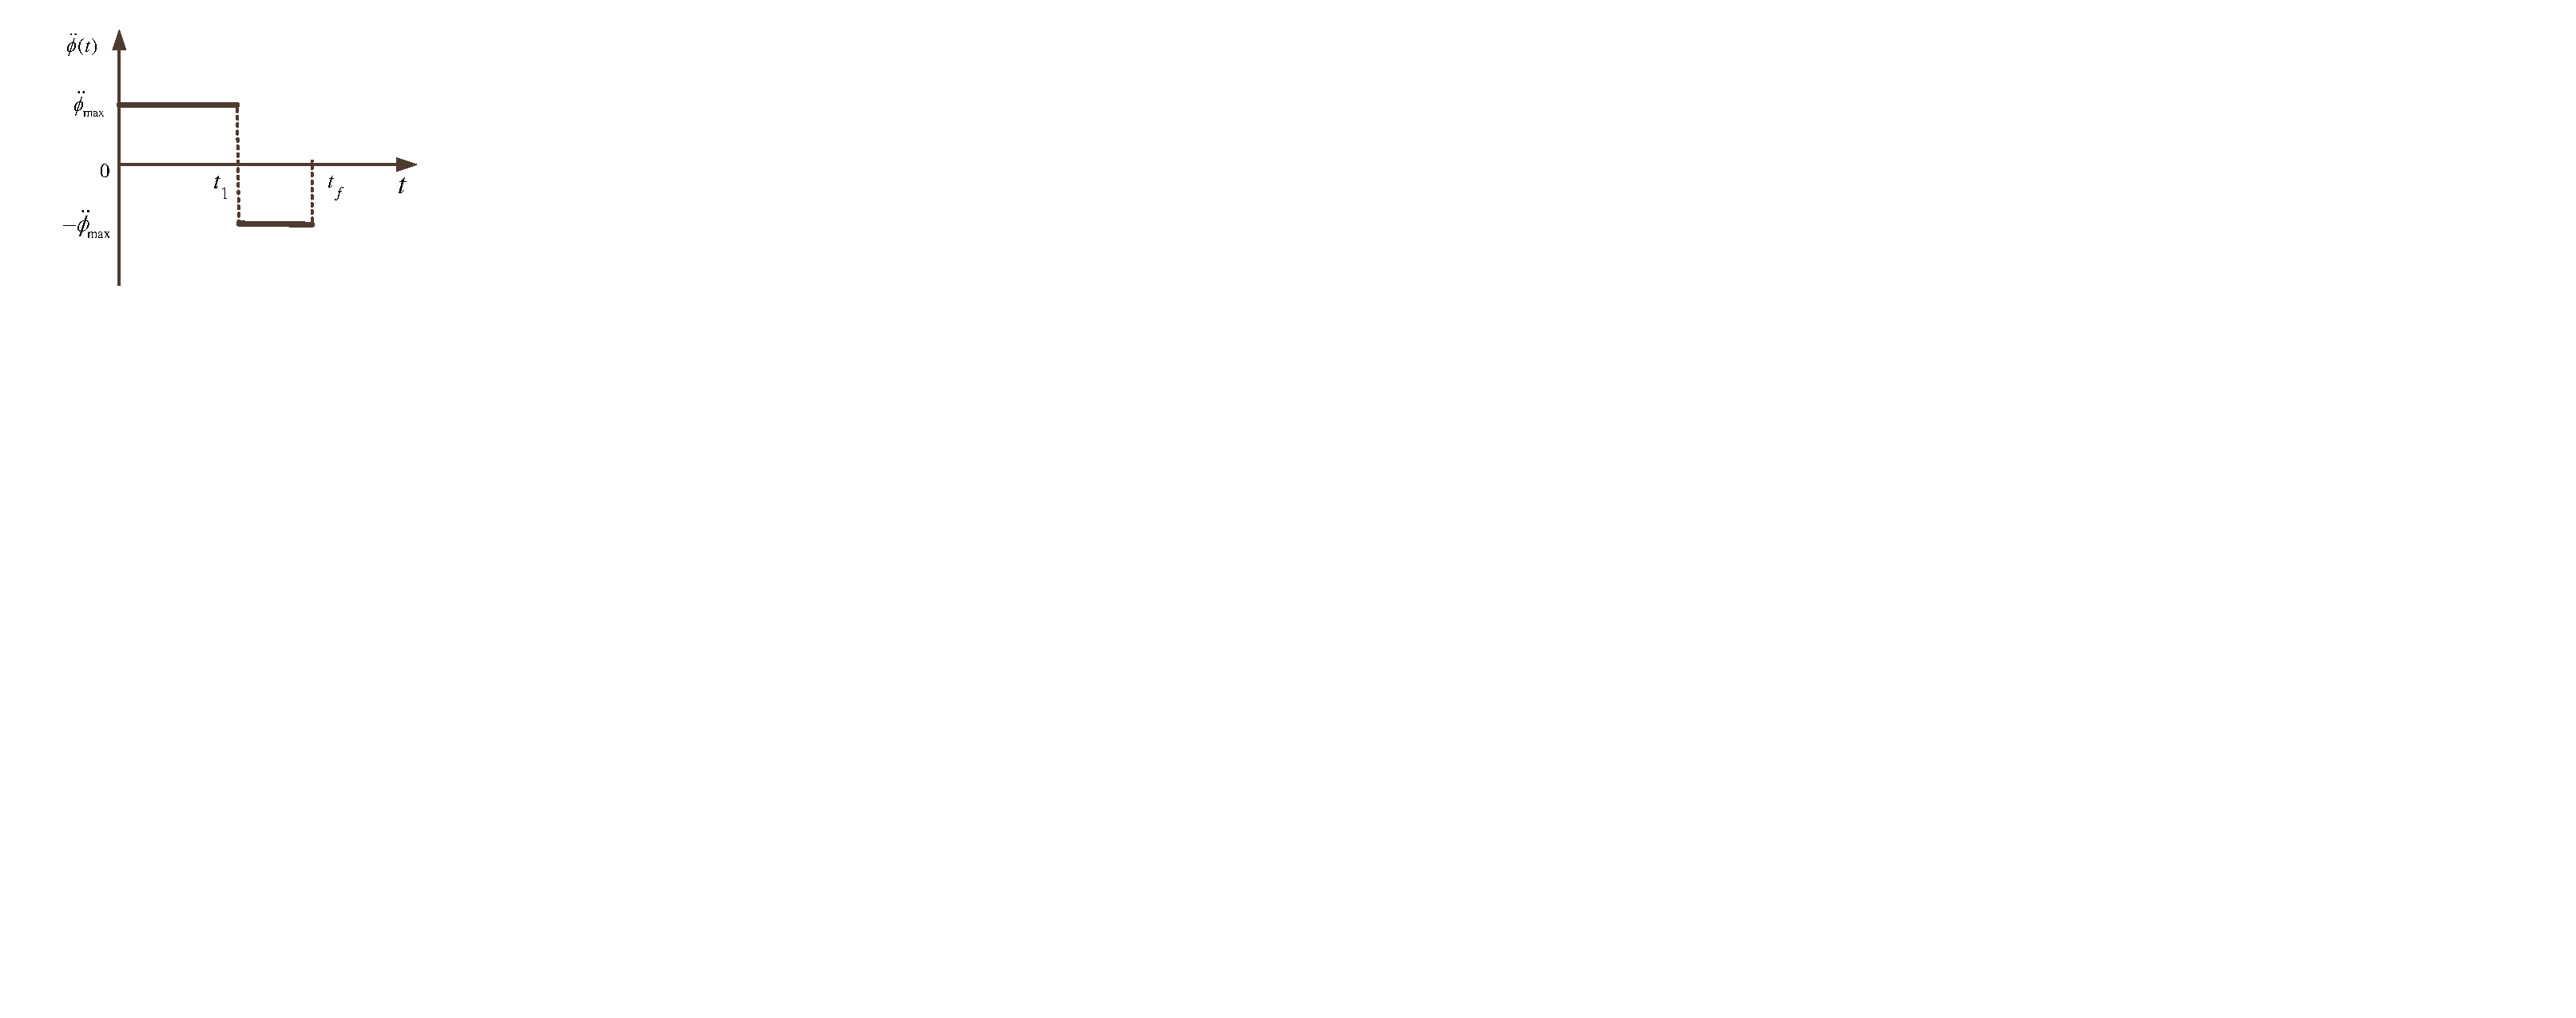
\includegraphics[width=2in]{./Figures/Bang_bang}    
	\caption{The optimal control in case 2.}  
	\label{bang_bang}
	\end{figure}
	where the switching and the final times are given by
	\begin{equation}
	t_1=t_0-\frac{\dot{\phi}_{0}}{\ddot{\phi}_{max}}+\frac{\sqrt{\ddot{\phi}_{max}^2(2\ddot{\phi}_{max}\phi_{f}+\dot{\phi}_{f}^2+\dot{\phi}_{0}^2)}}{\sqrt{2}\ddot{\phi}_{max}^2},
	\end{equation}
	
	%-------------------------------------------------------------------------------------------------------------------------------------------------------------------
	
	and
	\begin{equation}
	t_f=t_0-\frac{\dot{\phi}_{f}+\dot{\phi}_{0}}{\ddot{\phi}_{max}}+\frac{\sqrt{2}\sqrt{\ddot{\phi}_{max}^2(2\ddot{\phi}_{max}\phi_{f}+\dot{\phi}_{ef}^2+\dot{\phi}_{0}^2)}}{\ddot{\phi}_{max}^2}.
	\end{equation}
The angular velocity and angular rate about $\hat{e}$ axis are

	\begin{equation}\label{omega}
	\dot{\phi}(t)=\dot{\phi}_{0}+\ddot{\phi}_{max}(t-t_0)\mathbb{U}(t_0)- 2\ddot{\phi}_{max}(t-t_1)\mathbb{U}(t-t_1),
	\end{equation}

	\begin{equation}\label{phi}
	\phi(t)=\dot{\phi}_{0}(t-t_0)+\ddot{\phi}_{max}\frac{(t-t_0)^2}{2}\mathbb{U}(t_0)- 2\ddot{\phi}_{max}\frac{(t-t_1)^2}{2}\mathbb{U}(t-t_1).
	\end{equation}
	
	%-------------------------------------------------------------------------------------------------------------------------------------------------------------------
	
	%In the following, we calculate the $\phi(t)$, $\dot{\phi}(t)$, and $\ddot{\phi}(t)$ for each leg of the sun avoidance slew and from Eqs. (\ref{quatT})--(\ref{alpha_1}), we 
	\subsubsection{The First Slew Maneuver:} 
	This is a single-axis nonrest-to-rest maneuver around $\hat{e}$ with the boundary conditions

	\begin{equation}\label{Bc1}
	\dot{\phi}(t_0)=\dot{\phi}_{0},\phi(t_0)=0, \dot{\phi}(t_{f1})=0,\phi(t_{f1})=\phi_1.
	\end{equation}
	
	The switching time, $t_{11}$, and the minimum-time, $t_{f1}$, are 
	\begin{equation}\label{t11}
	t_{11}=t_0-\frac{\dot{\phi}_0}{\ddot{\phi}_{max}}+\frac{\sqrt{\ddot{\phi}_{max}^2(2\ddot{\phi}_{max}\phi_1+\dot{\phi}_{0}^2)}}{\sqrt{2}\ddot{\phi}_{max}^2},
	\end{equation}
	\begin{equation}\label{tf1}
	t_{f1}=t_0-\frac{\dot{\phi}_0}{\ddot{\phi}_{max}}+\frac{\sqrt{2\ddot{\phi}_{max}^2(2\ddot{\phi}_{max}\phi_1+\dot{\phi}_{0}^2)}}{\ddot{\phi}_{max}^2}.
	\end{equation}

	
	%-------------------------------------------------------------------------------------------------------------------------------------------------------------------
	
	\subsubsection{The Second Slew Maneuver:}
	This is a rest-to-rest maneuver around the sun vector with boundary conditions given by	
	\begin{equation}\label{Bc2}
	\dot{\phi}(t_0)=0, \phi(t_0)=0, \dot{\phi}(t_{f2})=0, \phi(t_{f2})=\phi_2.
	\end{equation}
	The switching time, $t_{12}$, and the minimum-time, $t_{f2}$, are
	\begin{equation}\label{t21}
	t_{12}=t_0-\frac{\sqrt{\phi_2}}{\ddot{\phi}_{max}},
	\end{equation}
	\begin{equation}\label{tf2}
	t_{f2}=t_0-\frac{2\sqrt{\phi_2}}{\ddot{\phi}_{max}}.
	\end{equation}

	
	%-------------------------------------------------------------------------------------------------------------------------------------------------------------------
	
	\subsubsection{The Third Slew Maneuver:}
	 This is a  single-axis rest-to-nonrest maneuver around $\hat{e}$ with the boundary conditions
	\begin{equation}\label{Bc3}
	\dot{\phi}(t_0)=0,\phi(t_0)=0, \dot{\phi}(t_{f3})=\dot{\phi}_{f},\phi(t_{f3})=\phi_3.
	\end{equation}
	The switching time, $t_{13}$, and the minimum-time, $t_{f3}$, are
	\begin{equation}\label{t31}
	t_{13}=t_0+\frac{\sqrt{\ddot{\phi}_{max}^2(2\ddot{\phi}_{max}\phi_3+\dot{\phi}_{f}^2)}}{\sqrt{2}\ddot{\phi}_{max}^2},
	\end{equation}
	\begin{equation}\label{tf3}
	t_{f3}=t_0-\frac{\dot{\phi}_{f}}{\ddot{\phi}_{max}}+\frac{\sqrt{2\ddot{\phi}_{max}^2(2\ddot{\phi}_{max}\phi_3+\dot{\phi}_{f}^2)}}{\ddot{\phi}_{max}^2}.
	\end{equation}
	Knowing the switching times for each slew, the $\ddot{\phi}(t)$, $\dot{\phi}(t)$, and  $\phi(t)$, can be found by substituting the boundary conditions for each slew into Eqs. (\ref{alpha}), (\ref{omega}), and (\ref{phi}), respectively. Then the slew plan, i.e. $^\mathcal{N}\omega^\mathcal{T}(t)$, $^\mathcal{N}\dot{\omega}^\mathcal{T}(t)$, $^\mathcal{N}q^\mathcal{T}(t)$, can be determined from Eqs. (\ref{quatT})--(\ref{k_omega}).	
	%-------------------------------------------------------------------------------------------------------------------------------------------------------------------
\section{Numerical simulation} 
We used MATLAB$^{\textregistered}$ to examine and validate the proposed algorithm in this paper. The initial, final, and sun position vectors were selected randomly such that the initial and final positions end up outside of the exclusion zone. The progression of the gyrostat along its orbit was not incorporated in these simulations, therefore, the sun vector does not change during the slew maneuvers. However, when the orbit is taken into account during real missions, the location of the sun vector during the $\phi_2$ portion of the maneuvers should be considered. Or rather, the timing of the instrument's LOS overlapping with the sun vector projection onto the slew plane should be used in the calculation of the slew angles. 
The pseudocode for the proposed SAS algorithm is shown Algorithm \ref{alg:pseudocode_slew}.   

\begin{algorithm}[h!]
	\caption{A Pseudocode for the SAS Algorithm}
	\label{alg:pseudocode_slew}
	\begin{algorithmic}[1]
		\State Find eigenaxis, $_\mathcal{N}e$ of slew plane 
		\State \hskip1.5em Compute cross product of $P_i$ and $P_f$ unit vectors 
		\State Compute angle between sun vector and slew plane angle $\alpha$ 
		\If{$|\alpha| < \epsilon_p$}
			\State Execute sun-avoidance slew: 
			\State \hskip1.5em Find $ \vec{S}_{||} $
			\State \hskip1.5em Compute $\phi_1$, $\phi_2$, $\phi_3$
			\State Compute $\phi_t$ 
		%		\For{each $\phi$}
		%		\State $\phi_1$: 
		\State Compute switching times $t_1$, $t_2$, $t_f$ for $\phi_1$, $\phi_2$, and $\phi_3$: 
		\If{$\phi > \phi_t$}
		\State Use equations (\ref{t1cons}) through (\ref{tfcons}) 
		\Else 
		\State Use equations (\ref{tfcons_phit}) through (\ref{t1cons_phit})
		\EndIf 
		\For{$t_0 < t < t_1$}
		\State Calculate inertial-to-desired rotation ${}^\mathcal{G}R^\mathcal{N}$
		\State From ${}^\mathcal{G}R^\mathcal{N}$, calculate $^\mathcal{N}\omega}^\mathcal{T}$, $^\mathcal{N}\dot{\omega}}^\mathcal{T}$ in the $\mathcal{G}$-frame
		\State \hskip1.5em Solve for control torque $u$ with equation (\ref{Euler_RBD1})
		\State \hskip1.5em Propagate $^\mathcal{N}\omega^\mathcal{G}$ and $^\mathcal{N}q^\mathcal{G}$ by solving equations (\ref{Euler_RBD}) and (\ref{kinematics}) 
		\EndFor 
		\State Repeat above lines for $t_1 < t < t_2$ and $t_2 < t < t_f$ 
		\Else 
			\State Slew directly from $P_i$ to $P_f$ 
		\EndIf 
	\end{algorithmic}
\end{algorithm}
In the following, we present the results of two cases: I) when the sun angle does not lie in the slew plane, $|\alpha|>0$, and II) when the sun vector lies in the slew plane, $\alpha=0$. The parameters used in both cases are listed in Table \ref{tab:alphaNot0_PiPfS_AWmax}. In case I, when $|\alpha|>0$, the gyrostat slews from the initial to the target position during the maneuvers, and $P_1$ and $P_2$ are connected via a rotation around the sun vector as shown in Fig.~\ref{fig:phi1_phi2_phi3}. The computed slew angles in this case are $(32.08, 102.56, 17.76)^\circ$.

\begin{table}[hbt!]
\centering
\caption{Initial, Final, and Sun Positions in Inertial Frame and Constraints Used in the Simulation}
\begin{tabular}{llccc}
\hline
Case&Symbol& Unit Vector & $\dot{\phi}_{max}$&$\ddot{\phi}_{max}$ \\
\hline
&$\hat{P}_i$ & $[-0.50, 0.57, 0.65]$& & \\
I)& $\hat{P}_f$ & $[0.76, -0.48, -0.44]$& $1\ (rad/s)$& $1\ (rad/s^2)$\\ 
&$\hat{S}$ & $[0.30, -0.50, -0.81]$& & \\
\hline
&$P_i$ & [0.65, -0.35, -0.67] & &\\
II)&$P_f$ & [-0.93, -0.25, 0.28] & $0.01\ (rad/s)$& $0.02\ (rad/s^2)$\\ 
&$S$ & [-0.20, -0.78, -0.59] & &\\
\hline
\end{tabular}
\label{tab:alphaNot0_PiPfS_AWmax}%
\end{table}
	\begin{figure}[hbt!]
	\centering
		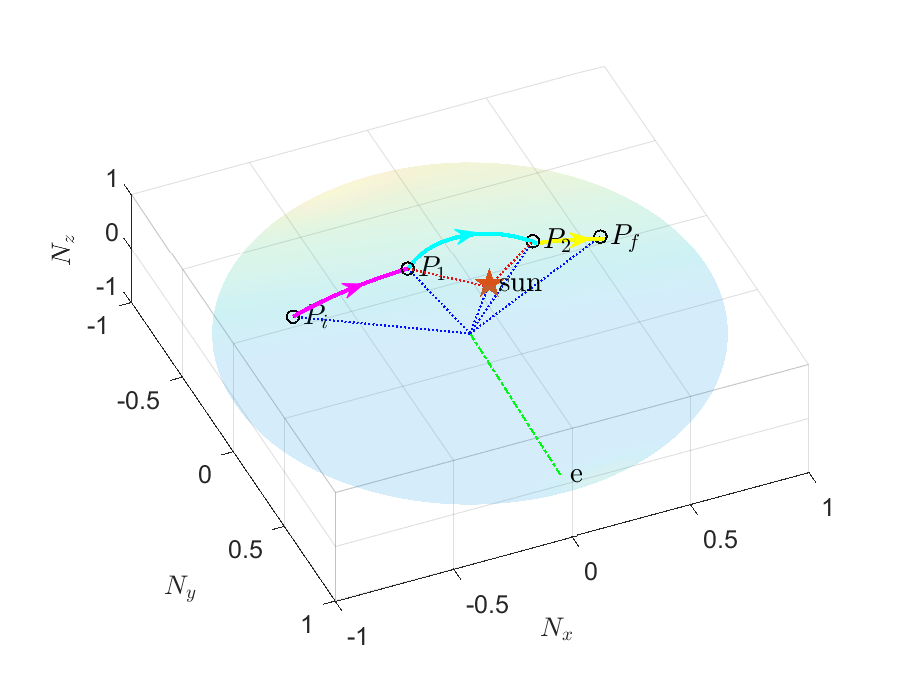
\includegraphics[width=4.75in]{figures/alphaNot0/phi1_phi2_phi3.eps}
		\caption{Trajectory of the tip of instrument's boresight during the entire slew when $|\alpha|>0$.}
		\label{fig:phi1_phi2_phi3}
\end{figure}	
The time histories of angular velocity and angular acceleration are shown in Fig. \ref{fig:ang_vel_acc}. In real missions, the gyrostat's reaction wheels' ability to impart angular momentum is translated to a constraint in angular velocity, and the thrusters ability to impose torque is translated to a constraint in angular acceleration. Therefore, no torque constraint is plotted in these results.
\begin{figure}[hbt!]
    \centering
    \begin{minipage}{.5\textwidth}
        \centering
    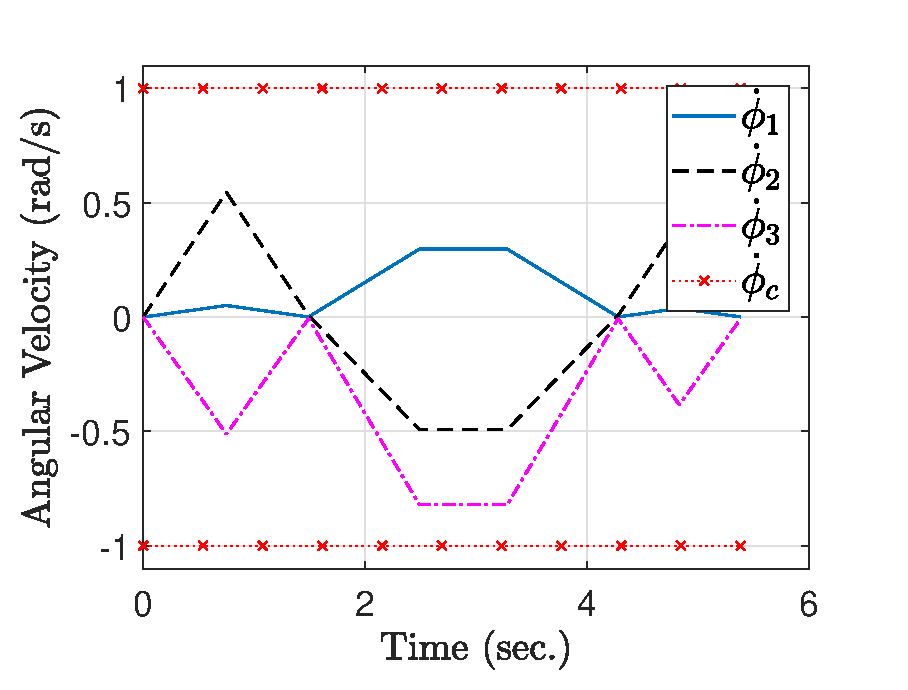
\includegraphics[width=3in]{figures/alphaNot0/ang_vel_phi_total.eps}
    \nocaption{a)}
    \end{minipage}%
    \begin{minipage}{0.5\textwidth}
        \centering
        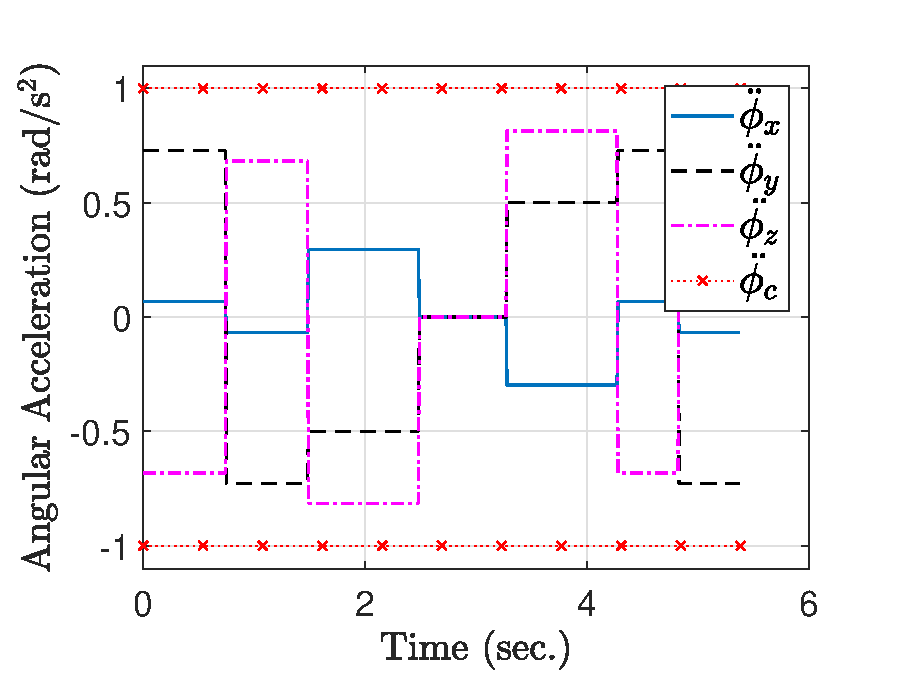
\includegraphics[width=3in]{figures/alphaNot0/ang_accel_total.eps}
       % \includegraphics[width=0.3\linewidth, height=0.15\textheight]{prob1_6_1}
       \nocaption{b)}
    \end{minipage}
    \caption{Time histories of gyrostat a) angular velocity and b) angular acceleration when $|\alpha|>0$.}
    \label{fig:ang_vel_acc} 
\end{figure}
Due to the high velocity and acceleration constraints, there is no coasting period for the $\phi_1$ and $\phi_3$ portions of the slew. However, there is a period of zero angular acceleration and constant angular velocity for $\phi_2$, which is reflected in Fig. \ref{fig:ang_vel_acc}. The time histories of quaternion and body-torque are shown in Fig. \ref{fig:quats_phi_total}.

\begin{figure}[htb!]
    \centering
    \begin{minipage}{.5\textwidth}
        \centering
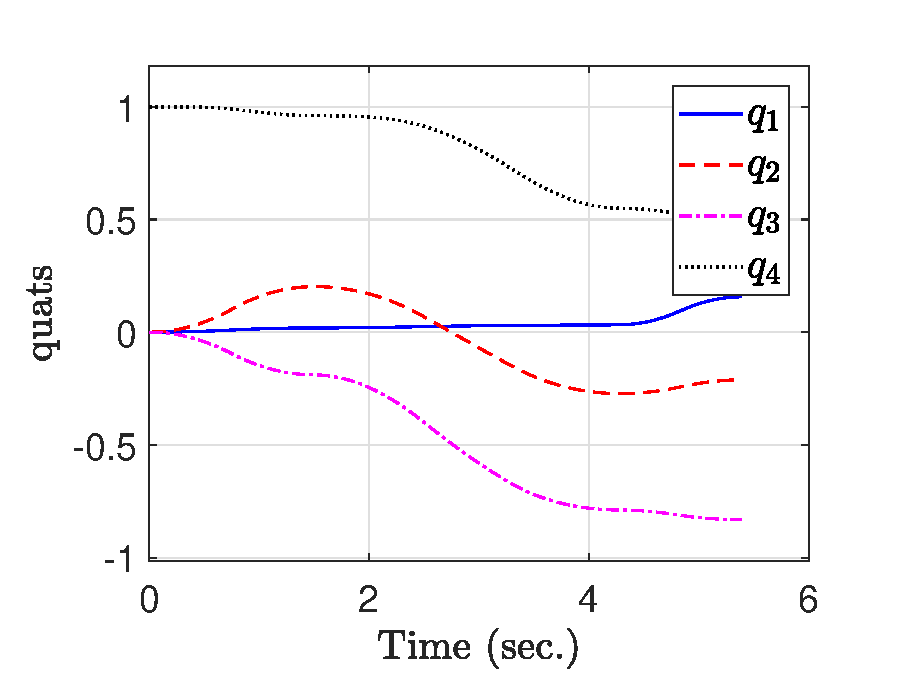
\includegraphics[width=3in]{figures/alphaNot0/quats_phi_total.eps}
    \nocaption{a)}
        \label{fig:prob1_6_2}
    \end{minipage}%
    \begin{minipage}{0.5\textwidth}
        \centering
   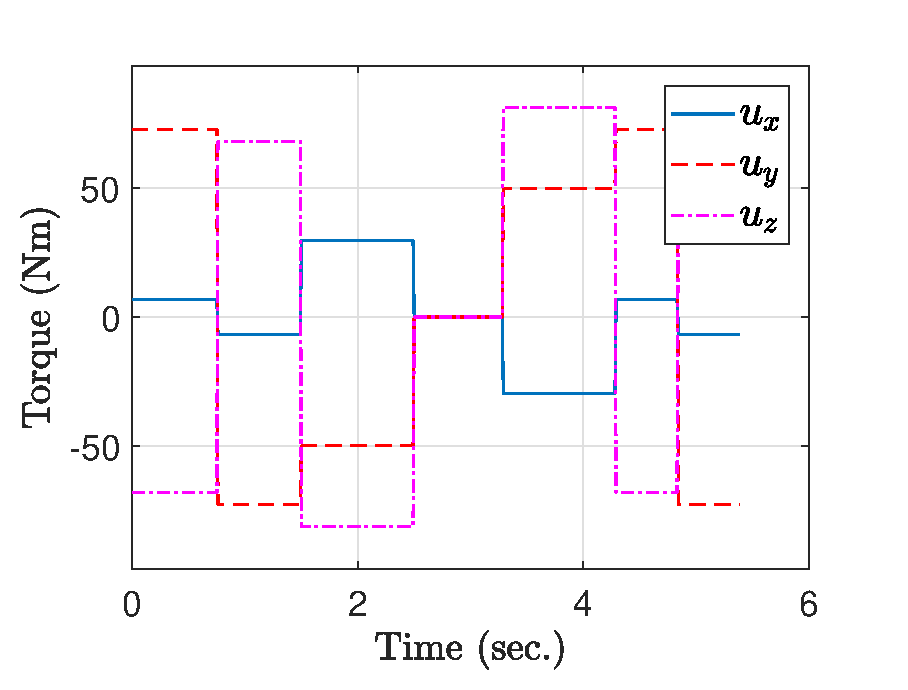
\includegraphics[width=3in]{figures/alphaNot0/torque_total.eps}
       % \includegraphics[width=0.3\linewidth, height=0.15\textheight]{prob1_6_1}
        \label{fig:prob1_6_1}
       \nocaption{b)}
    \end{minipage}
    \caption{Time histories of a) gyrostat-frame quaternions and b) body torques when $|\alpha|>0$.}
    \label{fig:quats_phi_total}
	\end{figure}
	
In case II,  when $\alpha=0$, we choose much more realistic constraints: 0.01 rad/s for angular velocity and 0.01 rad/s$^2$ for angular acceleration. The computed slew angles in this case are $(41.82, 180, 62.45)^\circ$. The trajectory of the instrument's LOS is shown in Fig. ~\ref{fig:phi1_phi2_phi3_alpha0}.
\begin{figure}[!h]
\centering
		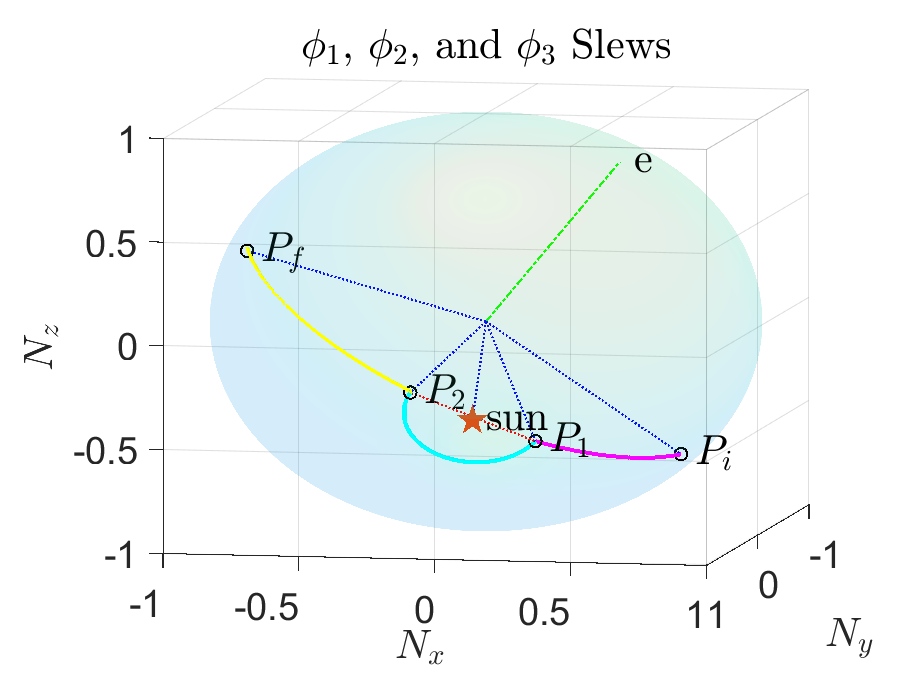
\includegraphics[width=4.75in]{figures/alpha0/alpha0_phi1_phi2_phi3.eps}		
\caption{Trajectory of the tip of instrument's boresight during the entire slew when $\alpha=0$.}
\label{fig:phi1_phi2_phi3_alpha0}
\end{figure}	
With smaller constraints, the simulation takes much longer to complete the slew maneuvers. Figs. ~\ref{fig:ang_vel_acc0} and \ref{fig:quats_phi_total0} show that the torque and acceleration applied are very short compared to the duration of the entire maneuver for case I ($|\alpha| > 0$), in contrast to Figs. ~\ref{fig:ang_vel_acc} and \ref{fig:quats_phi_total} for case II ($\alpha = 0$). The gyrostat spends the majority of the time coasting at constant angular velocity, as seen in Fig. ~\ref{fig:ang_vel_acc0}. Though the initial and final points are further apart in the gyrostat unit sphere to begin with, the simulation takes an order of magnitude longer to complete at almost $500$ seconds for $\alpha = 0$, as opposed to about $5.5$ seconds for $|\alpha| > 0$. The case shown here is much more realistic example that reflects real-world conditions. The results for both cases demonstrate that the angular velocity and acceleration never exceed the velocity and acceleration constraints for any axis.
\begin{figure}[htb!]
    \centering
    \begin{minipage}{.5\textwidth}
        \centering
  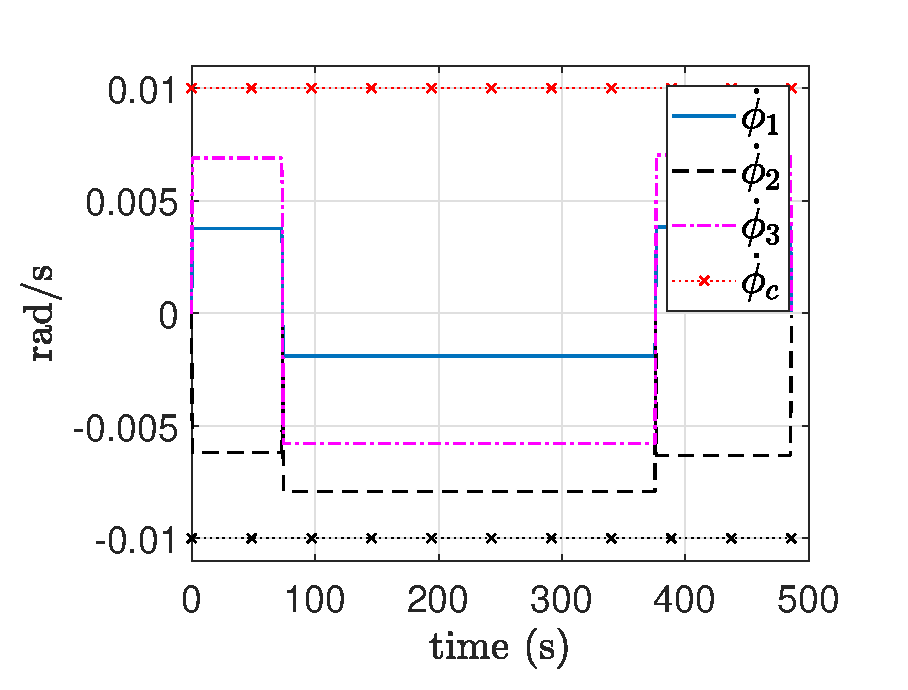
\includegraphics[width=3in]{figures/alpha0/ang_vel.eps}
    \nocaption{a)}
    \end{minipage}%
    \begin{minipage}{0.5\textwidth}
        \centering
       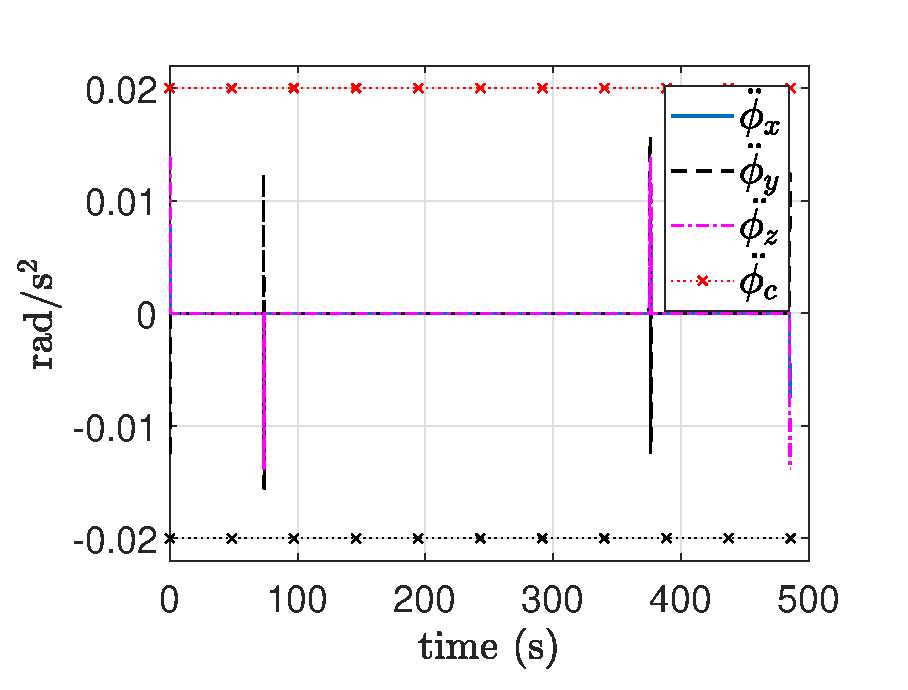
\includegraphics[width=3in]{figures/alpha0/ang_accel.eps}
       % \includegraphics[width=0.3\linewidth, height=0.15\textheight]{prob1_6_1}
       \nocaption{b)}
    \end{minipage}
    \caption{Time histories of gyrostat a) angular velocity and b) angular acceleration when $\alpha=0$.}
    \label{fig:ang_vel_acc0} 
\end{figure}

\begin{figure}[htb!]
    \centering
    \begin{minipage}{.5\textwidth}
        \centering
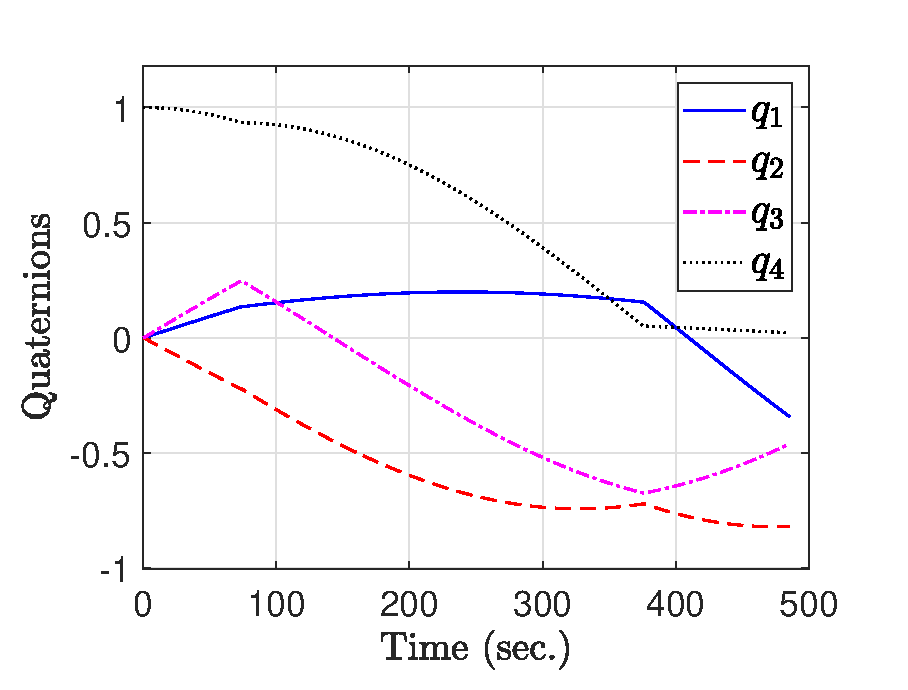
\includegraphics[width=3in]{figures/alpha0/quats.eps}
    \nocaption{a)}
    \end{minipage}%
    \begin{minipage}{0.5\textwidth}
        \centering
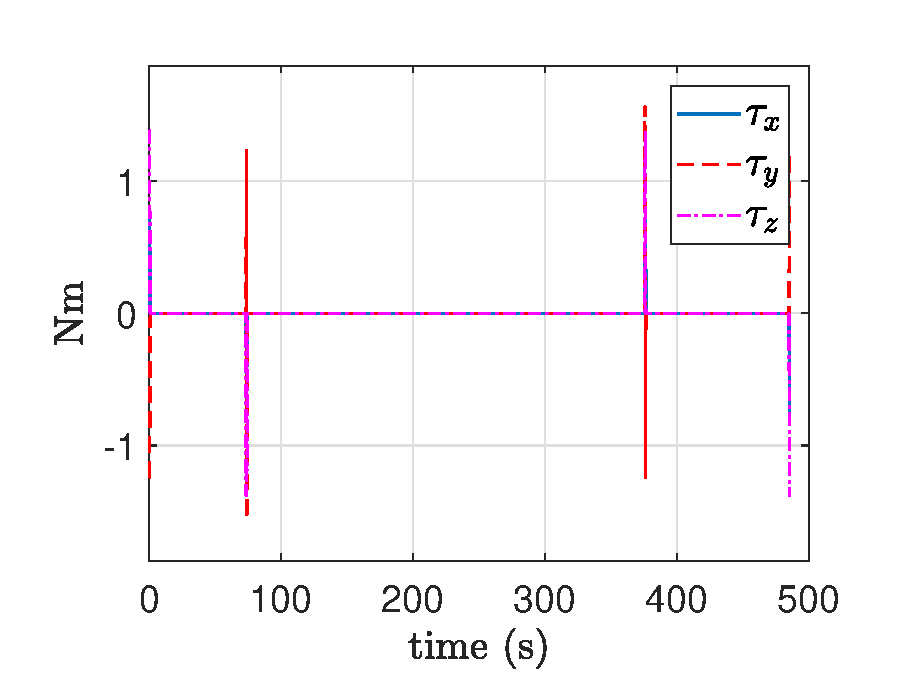
\includegraphics[width=3in]{figures/alpha0/torque.eps}
       \nocaption{b)}
    \end{minipage}
    \caption{Time histories of a) gyrostat-frame quaternions and b) body torques when $\alpha=0$.}
    \label{fig:quats_phi_total0}
	\end{figure}
			
	
%%%%%%%%%%%%
			
%%%%%%%%%%%%
	\newpage
	\section{Conclusion}
	 A new geometric approach for large-angle slew planning with pointing and actuator constraints is presented. The gyrostat has a single light-sensitive payload with control-torque and reaction wheels' angular momentum constraints. Furthermore, we assume that the initial and final attitudes, instrument's line-of-sight vector, and sun vector are known. Then the quaternions, angular velocities, and angular accelerations of the desired or target frame are derived based on the PMP.  The proposed algorithm is intuitive, closed-form, and easy to implement. The main drawback of the proposed algorithm is its limitation for a single sensitive-payload. The feasibility of the proposed algorithm is demonstrated for two arbitrary cases and it has been investigated via extensive numerical simulations.
	\section{Acknowledgment}
	This research is supported by Maxar Space Infrastructure (Formerly Space Systems/Loral). The second author would like to acknowledge Luke DeGalan for his useful comments.

	


	
	\bibliographystyle{AAS_publication}   % Number the references.
	\bibliography{references_SAA}   % Use references.bib to resolve the labels.
	
	
	
\end{document}
